\documentclass[11pt]{article}

% ---------- Paquetes ----------
\usepackage[spanish,es-noshorthands]{babel}
\usepackage[utf8]{inputenc}
\usepackage[T1]{fontenc}
\usepackage[margin=2.5cm]{geometry}
\usepackage{graphicx}
\usepackage{booktabs}
\usepackage{longtable}
\usepackage{array}
\usepackage{caption}
\usepackage{float}
\usepackage{xcolor}
\usepackage[colorlinks=true, linkcolor=black, citecolor=black, urlcolor=blue]{hyperref}
\usepackage{parskip}
\usepackage{fancyhdr}

% Todas las imagenes viven en img/, junto a este .tex, dentro de docs/
\graphicspath{{img/}}
\setlength{\headheight}{14pt}
\setlength{\parindent}{0pt}
\setlength{\parskip}{6pt}

\pagestyle{fancy}
\fancyhf{}
\fancyhead[L]{Laboratorio 4 -- Datos Geoespaciales}
\fancyhead[R]{CC3084 -- Data Science}
\fancyfoot[C]{\thepage}
\renewcommand{\headrulewidth}{0.4pt}

\title{\vspace{-1.5cm}\textbf{Floraciones de cianobacterias en los lagos de Atitl\'an y Amatitl\'an}\\
\large Monitoreo satelital con im\'agenes Sentinel-2}
\author{
  Javier España \#23361 \and
  Angel Esquit \#23221 \and
  Roberto Barreda \#23354
}
\date{Universidad del Valle de Guatemala \\ Facultad de Ingenier\'ia -- CC3084 Data Science \\ Semestre II, 2026}

\begin{document}

\maketitle
\thispagestyle{empty}

\begin{abstract}
\noindent Este informe resume el monitoreo de floraciones de cianobacterias en los lagos de Atitl\'an y Amatitl\'an durante el per\'iodo enero 2025 -- julio 2026, a partir de 22 im\'agenes del sat\'elite Sentinel-2 (11 fechas por lago). Se reprodujo el \emph{Cyano Detection Script} publicado en el repositorio de Sentinel Hub para estimar la concentraci\'on de clorofila-a, un indicador indirecto de la cantidad de algas y cianobacterias presentes en el agua, y se complement\'o con los \'indices NDVI y NDWI. Los resultados muestran dos lagos en estados muy distintos: Amatitl\'an presenta una eutrofizaci\'on cr\'onica, con un promedio de clorofila-a 5.3 veces mayor que Atitl\'an y un evento de floraci\'on generalizada en junio de 2026 que cubri\'o cerca del 77\,\% de su superficie. Atitl\'an, en cambio, se mantiene en un estado saludable a nivel de lago completo, aunque con focos puntuales de concentraci\'on alta cerca de algunas bah\'ias.
\end{abstract}

\tableofcontents

% ======================================================================
\section{Introducci\'on}
% ======================================================================

Los lagos de Atitl\'an y Amatitl\'an son dos de los cuerpos de agua m\'as importantes de Guatemala, tanto por su valor ecol\'ogico y tur\'istico como por los servicios que prestan a las comunidades que dependen de ellos. En las \'ultimas d\'ecadas, ambos han mostrado signos de deterioro ambiental, en particular por la proliferaci\'on de cianobacterias: microorganismos que, bajo ciertas condiciones (agua c\'alida, exceso de nutrientes, poca circulaci\'on), pueden formar floraciones capaces de producir toxinas da\~ninas para la salud humana y para la vida acu\'atica.

Monitorear estas floraciones mediante muestreos f\'isicos en el lago es costoso, lento y limitado a los puntos donde efectivamente se toma la muestra. La observaci\'on satelital ofrece una alternativa complementaria: la misi\'on Sentinel-2 del programa Copernicus captura im\'agenes multiespectrales de todo el planeta cada pocos d\'ias, con una resoluci\'on suficiente para distinguir zonas de un lago con distinta concentraci\'on de algas.

El objetivo de este trabajo fue utilizar im\'agenes Sentinel-2 para estimar, en un conjunto fijo de 11 fechas por lago (definidas por el enunciado del laboratorio), un \'indice de cianobacteria para Atitl\'an y Amatitl\'an, analizar c\'omo evoluciona ese \'indice en el tiempo y en el espacio, y comparar el comportamiento de ambos lagos para identificar posibles causas de sus diferencias.

% ======================================================================
\section{De d\'onde salen los datos y c\'omo se procesaron}
% ======================================================================

Esta secci\'on explica, en t\'erminos generales y sin entrar en c\'odigo, qu\'e datos se usaron y qu\'e c\'alculos se les aplicaron. El detalle t\'ecnico completo, con el c\'odigo en Python, est\'a disponible en el repositorio del proyecto.

\subsection{Im\'agenes satelitales utilizadas}

Se descargaron im\'agenes del sat\'elite Sentinel-2 (producto L2A, ya corregido atmosf\'ericamente) a trav\'es de la plataforma \emph{Copernicus Data Space Ecosystem}, usando el m\'odulo \texttt{openEO} para pedir \'unicamente las bandas espectrales necesarias en lugar de escenas completas. Esto redujo el peso de cada descarga de varios cientos de megabytes a apenas unos pocos, sin perder la informaci\'on necesaria para los \'indices que se calculan m\'as adelante.

Siguiendo las fechas oficiales fijadas en el enunciado del laboratorio, se trabaj\'o con \textbf{11 fechas por lago} (22 im\'agenes en total), todas con nubosidad baja, entre enero de 2025 y julio de 2026. Para cada fecha se descargaron nueve bandas espectrales (de la azul hasta el infrarrojo de onda corta), recortadas al \'area de cada lago y remuestreadas a 20 metros de resoluci\'on espacial, es decir, cada p\'ixel de las im\'agenes representa un cuadro de 20x20 metros sobre la superficie del lago.

\subsection{El \'indice de cianobacteria}

Para estimar la presencia de cianobacterias se reprodujo en Python el \emph{Cyano Detection Script} (\texttt{cyanobacteria\_chla\_ndci\_l1c}), publicado en el repositorio p\'ublico de scripts de Sentinel Hub. El script combina tres ideas:

\begin{itemize}
    \item \textbf{Identificar qu\'e p\'ixeles son agua.} No toda la escena descargada es lago: hay orilla, suelo y zonas urbanas cercanas que deben excluirse. El script aplica varios criterios espectrales combinados para separar el agua del resto.
    \item \textbf{Estimar la clorofila-a.} La clorofila-a es el pigmento que le da el color verde a las algas y cianobacterias; su concentraci\'on (medida en mg/m\textsuperscript{3}) es el indicador que se usa en este informe como \emph{\'indice de cianobacteria}. Se calcula a partir de un \'indice espectral llamado NDCI (que compara dos bandas del rojo y el borde rojo del espectro) mediante una f\'ormula de calibraci\'on emp\'irica publicada por los autores del script original.
    \item \textbf{Detectar vegetaci\'on o natas flotantes.} Un tercer \'indice (FAI) permite distinguir manchas de vegetaci\'on o espuma que flotan en la superficie, separ\'andolas de la clorofila disuelta en el agua.
\end{itemize}

El script fue calibrado originalmente con im\'agenes sin corregir atmosf\'ericamente (L1C); en este trabajo se aplic\'o sobre im\'agenes ya corregidas (L2A), que son m\'as estables entre fechas y sat\'elites distintos. Esto implica que los valores en mg/m\textsuperscript{3} deben interpretarse como una escala \textbf{relativa}, \'util para comparar fechas y zonas entre s\'i, y no como una medici\'on de laboratorio calibrada al mil\'imetro.

Adem\'as del \'indice de cianobacteria, se calcularon dos \'indices adicionales solicitados en el enunciado:

\begin{itemize}
    \item \textbf{NDVI}, normalmente usado para vegetaci\'on terrestre, pero que sobre agua con algas tiende a subir cuando hay m\'as biomasa.
    \item \textbf{NDWI}, que mide cu\'anta agua limpia hay en la escena; tiende a bajar cuando el agua est\'a cargada de pigmentos.
    \item se calcularon \'unicamente sobre los p\'ixeles que el an\'alisis identific\'o como agua.
\end{itemize}

\subsection{Una ``huella'' fija para poder comparar fechas}

Un problema pr\'actico surgi\'o al aplicar el script de identificaci\'on de agua fecha por fecha: cuando hay una floraci\'on muy densa, el agua se ve turbia y verdosa, y el propio criterio que identifica el agua puede dejar de reconocer esos p\'ixeles como agua, precisamente porque el agua ya no ``parece'' agua limpia. Esto sub-estimar\'ia justo los eventos que interesa detectar, y adem\'as har\'ia que el \'area sobre la que se promedia cambiara de una fecha a otra.

Para evitarlo se defini\'o una \textbf{huella fija de cada lago}: la zona que el criterio de agua reconoce como tal en al menos el 30\,\% de las 11 fechas, despu\'es de rellenar huecos peque\~nos y quedarse solo con el cuerpo de agua principal (sin islas sueltas de p\'ixeles mal clasificados). Todas las estad\'isticas de este informe se calculan sobre esa misma huella para cada lago, lo que permite comparar fechas de manera justa. La huella obtenida fue de \textbf{13.8 km\textsuperscript{2}} para Amatitl\'an y \textbf{120.8 km\textsuperscript{2}} para Atitl\'an, valores cercanos a la superficie oficial de cada lago (15.2 y 130.1 km\textsuperscript{2}, respectivamente; la diferencia corresponde sobre todo a la franja costera de p\'ixeles mixtos agua-tierra, que se excluye a prop\'osito).

Una \'unica fecha, Atitl\'an 2025-01-18, se descart\'o de los an\'alisis de tendencia por tener muy poca cobertura v\'alida dentro de la huella (23.4\,\%): en esa imagen la correcci\'on atmosf\'erica devolvi\'o reflectancias sin sentido en una parte grande del lago, probablemente por la profundidad y oscuridad del agua en esa zona.

% ======================================================================
\section{El \'indice de cianobacteria sobre el mapa}
% ======================================================================

Antes de analizar tendencias, conviene ver c\'omo se ve el \'indice sobre el mapa. La Figura~\ref{fig:mapas_amatitlan} muestra Amatitl\'an en su fecha m\'as limpia del per\'iodo (2026-02-02) y en su fecha de mayor floraci\'on (2026-06-19); la Figura~\ref{fig:mapas_atitlan} muestra el mismo contraste para Atitl\'an. En cada figura, el primer panel es una imagen de color real (lo que ver\'ia el ojo humano desde el sat\'elite), el segundo muestra qu\'e p\'ixeles identific\'o el script como agua ese d\'ia, y los dos \'ultimos muestran el NDCI y la clorofila-a estimada, con la misma rampa de colores oficial del script: azul es agua limpia, verde es biomasa moderada, y amarillo/naranja es floraci\'on densa.

\begin{figure}[H]
    \centering
    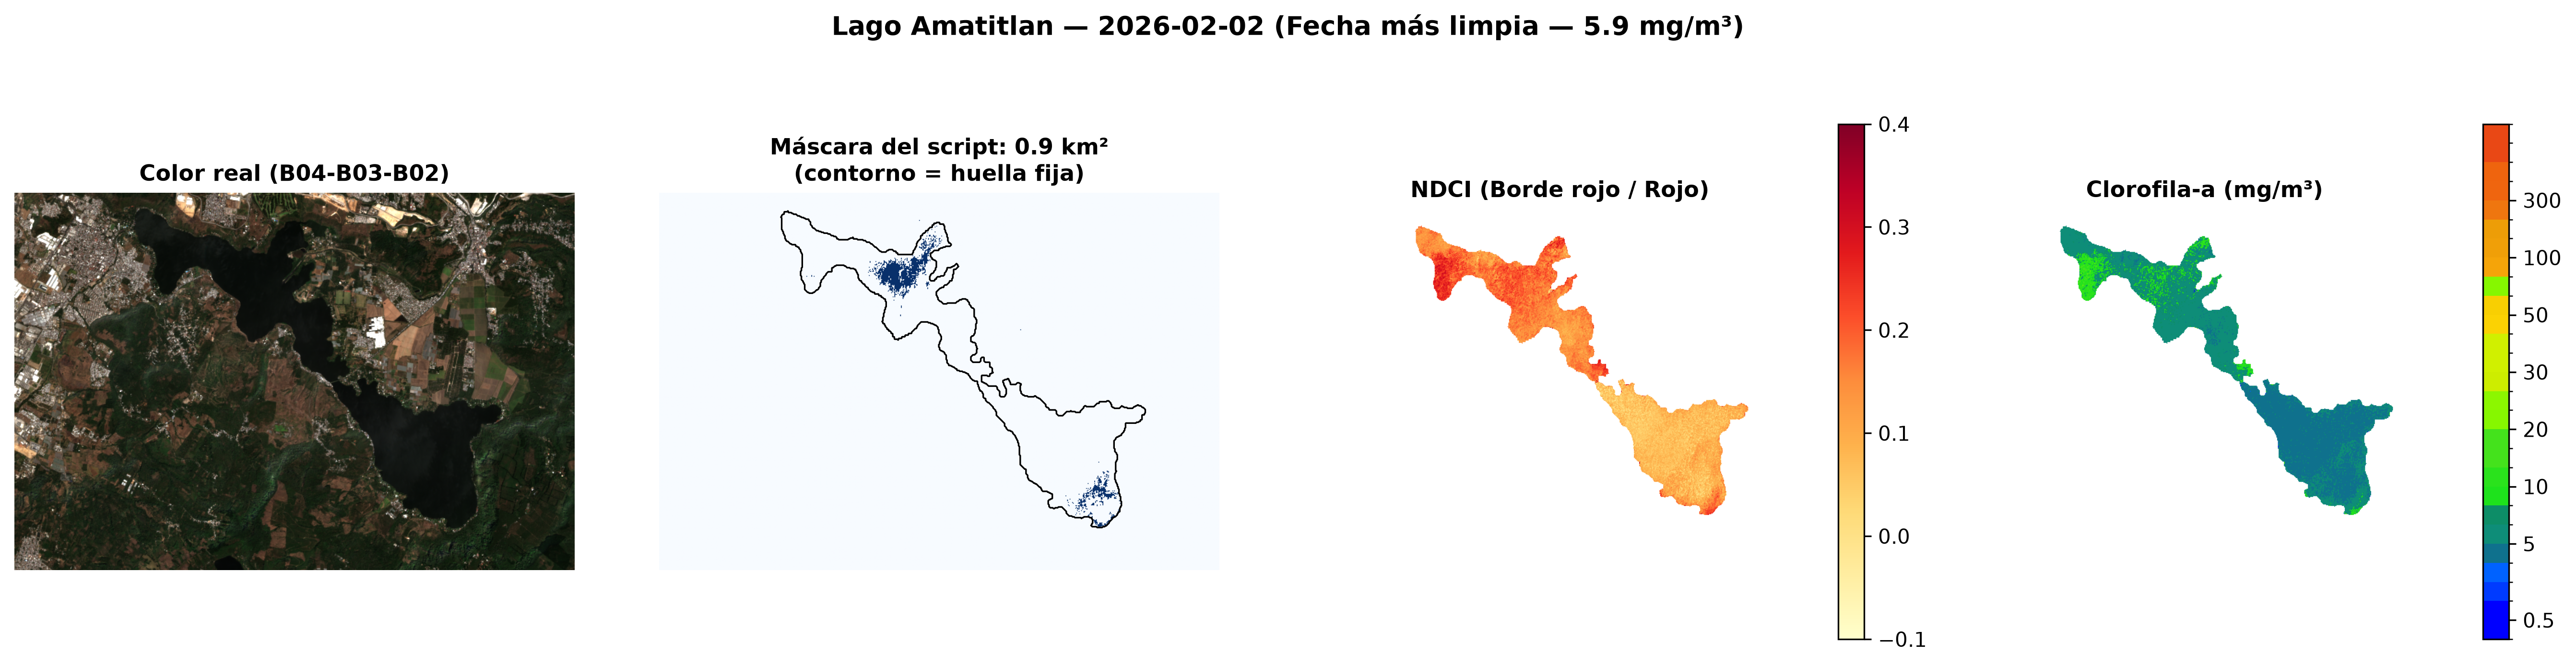
\includegraphics[width=\textwidth]{mapa_amatitlan_limpia.png}
    \vspace{4pt}
    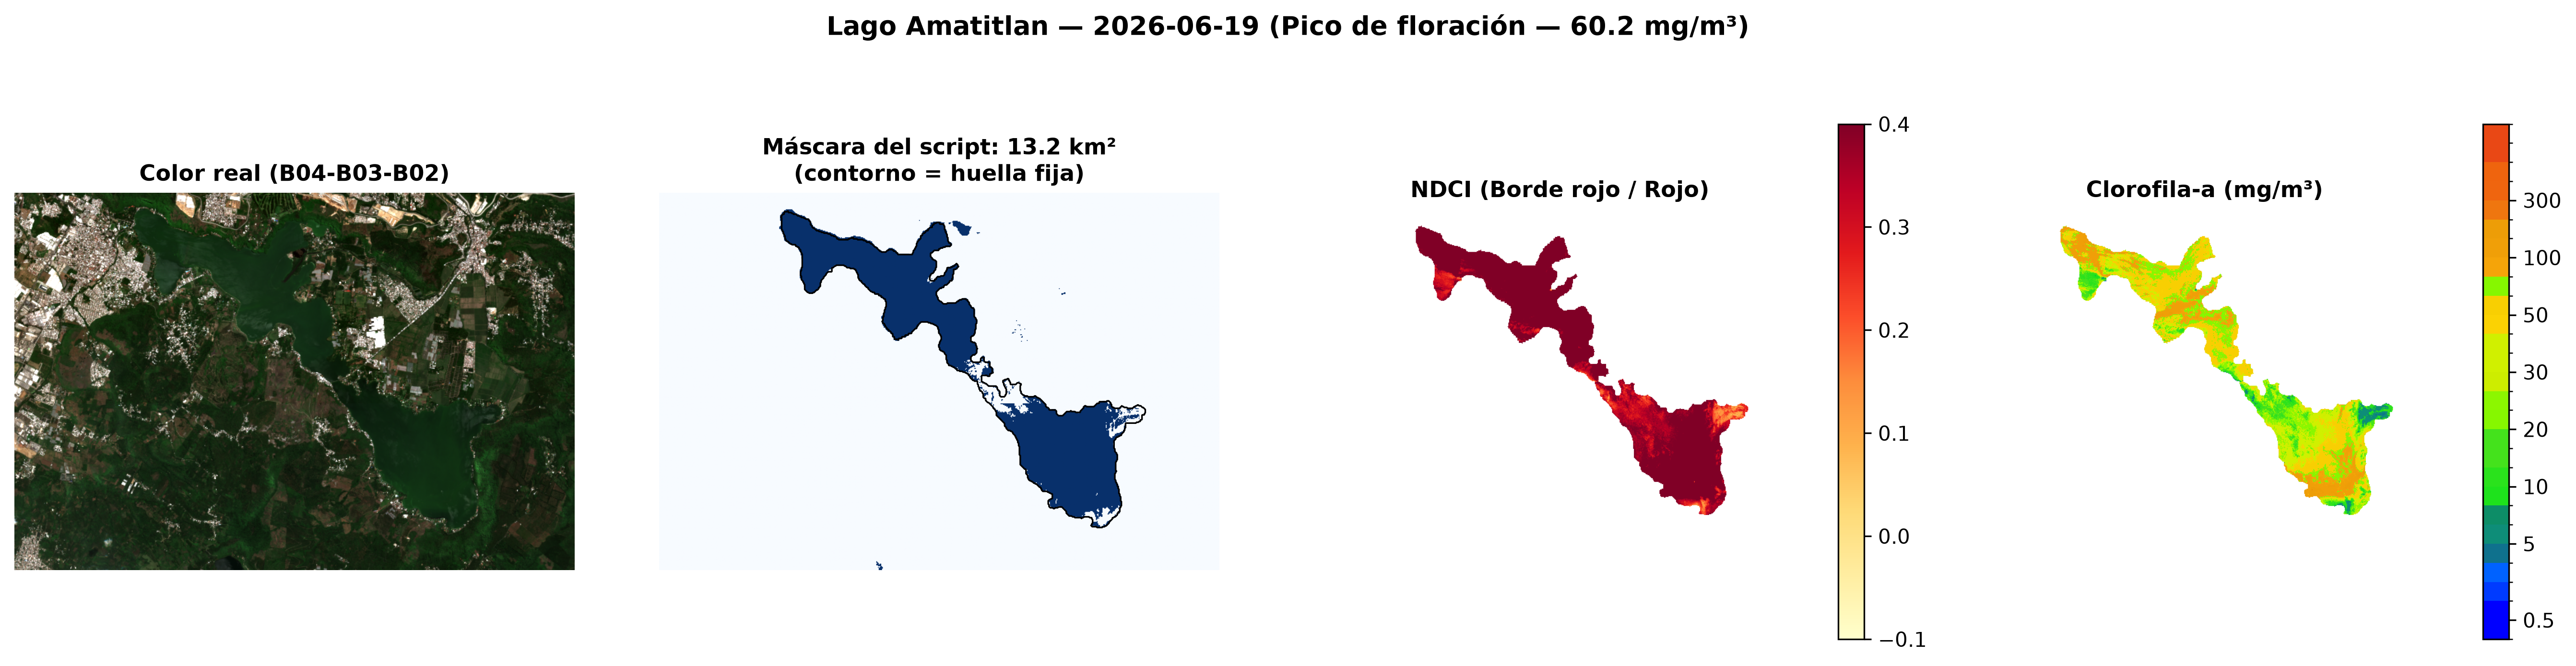
\includegraphics[width=\textwidth]{mapa_amatitlan_pico.png}
    \caption{Lago Amatitl\'an: fecha m\'as limpia del per\'iodo (arriba, 2026-02-02, 5.9 mg/m\textsuperscript{3} de clorofila-a promedio) frente a la fecha de mayor floraci\'on (abajo, 2026-06-19, 60.2 mg/m\textsuperscript{3}). En la imagen de color real de la fecha con floraci\'on se aprecia a simple vista el tono verdoso del agua.}
    \label{fig:mapas_amatitlan}
\end{figure}

\begin{figure}[H]
    \centering
    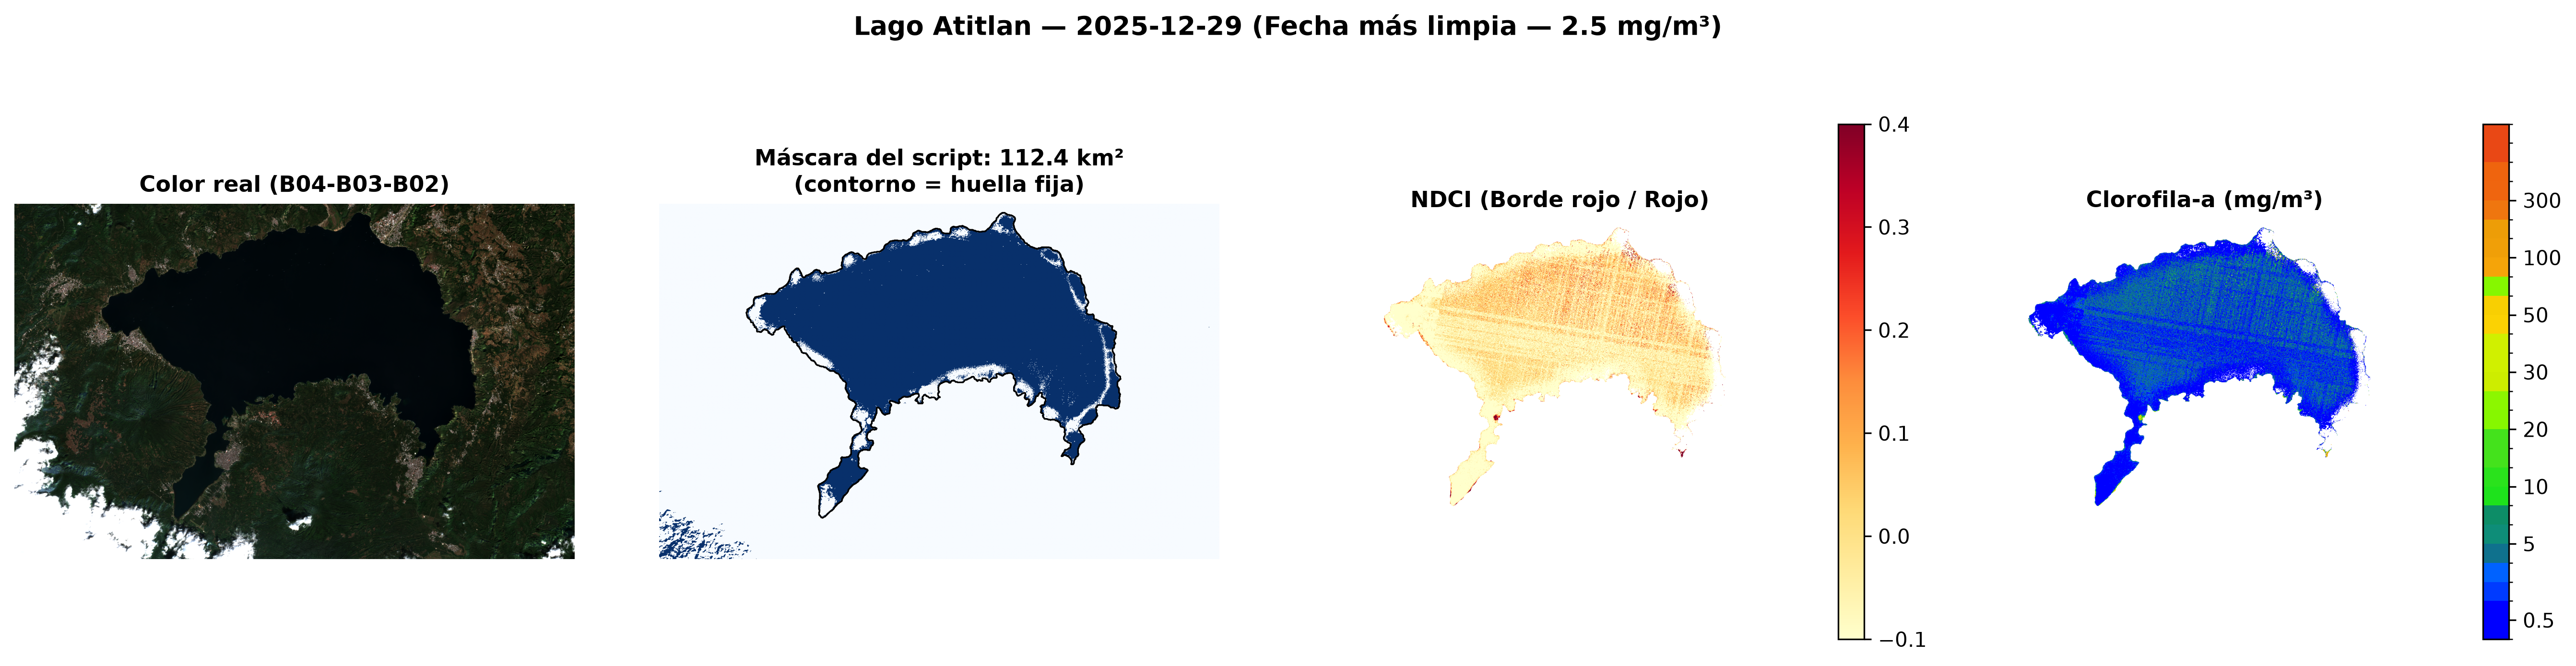
\includegraphics[width=\textwidth]{mapa_atitlan_limpia.png}
    \vspace{4pt}
    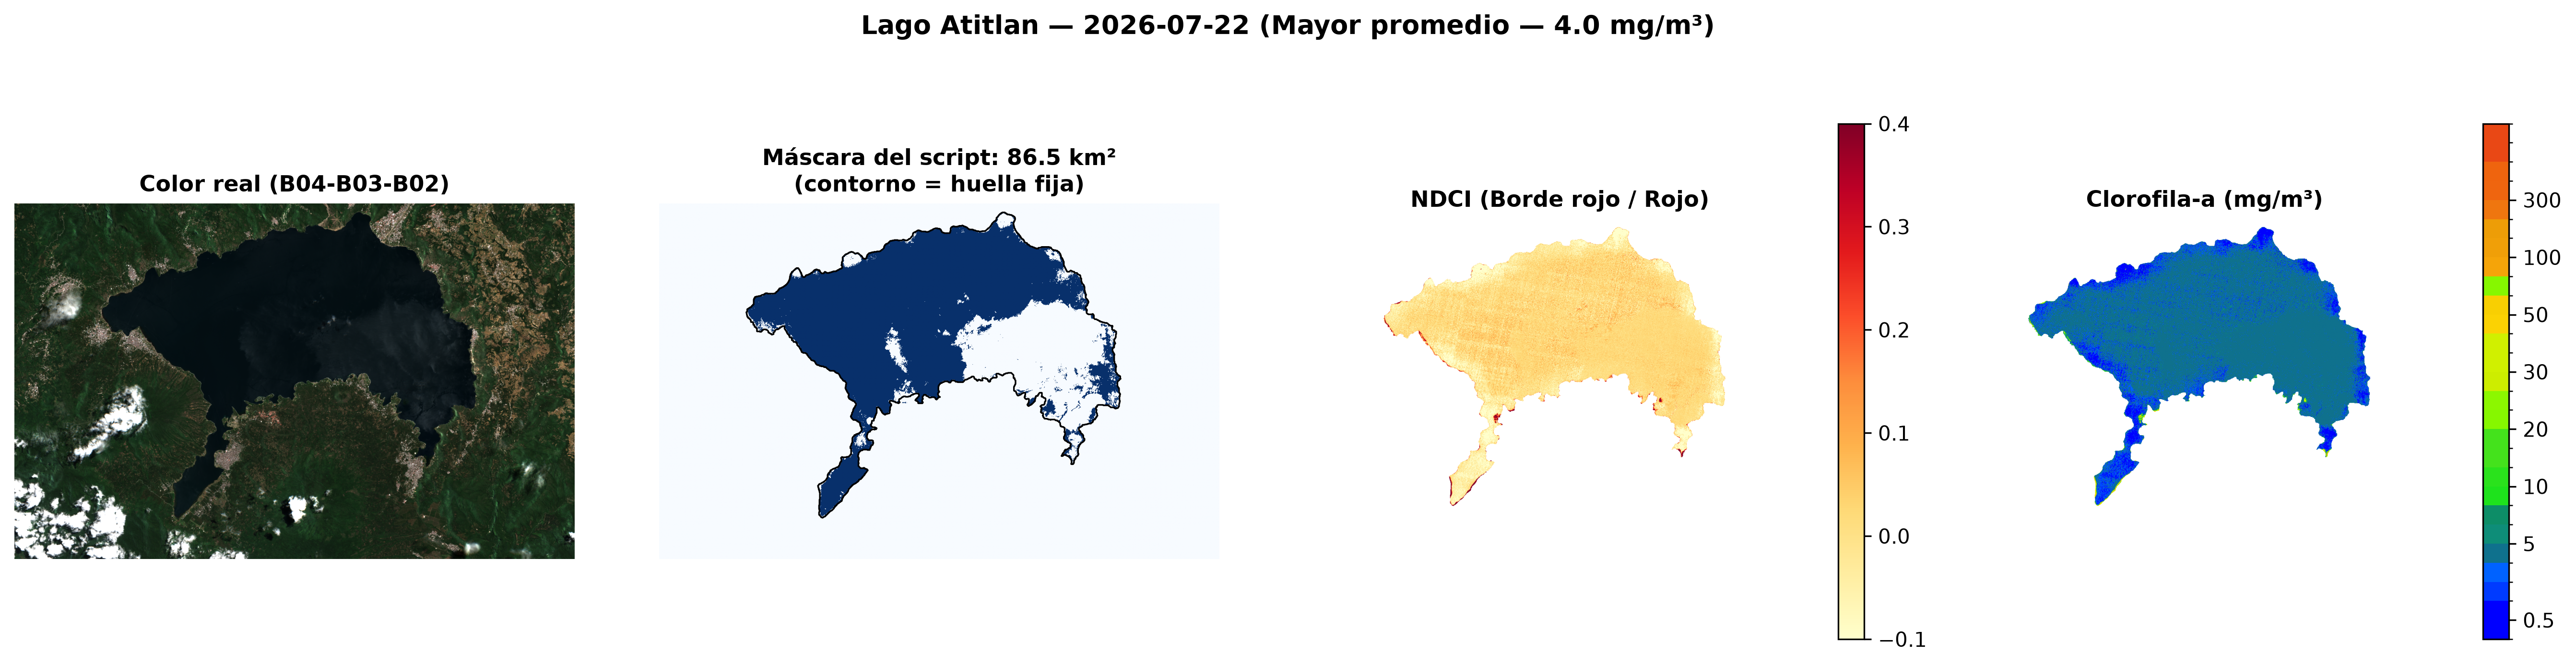
\includegraphics[width=\textwidth]{mapa_atitlan_pico.png}
    \caption{Lago Atitl\'an: fecha m\'as limpia del per\'iodo (arriba, 2025-12-29, 2.5 mg/m\textsuperscript{3}) frente a la fecha con mayor promedio (abajo, 2026-07-22, 4.0 mg/m\textsuperscript{3}). Ntese que la escala de colores es la misma que en Amatitl\'an: incluso en su ``peor'' fecha, Atitl\'an se mantiene casi todo en tonos azules.}
    \label{fig:mapas_atitlan}
\end{figure}

Ya en esta comparaci\'on inicial se nota la diferencia de fondo entre los dos lagos: la fecha de mayor floraci\'on de Atitl\'an (4.0 mg/m\textsuperscript{3}) es m\'as baja que la fecha \emph{m\'as limpia} de Amatitl\'an (5.9 mg/m\textsuperscript{3}).

% ======================================================================
\section{An\'alisis temporal}
% ======================================================================

\subsection{Evoluci\'on de la clorofila-a}

Para cada fecha se calcul\'o el promedio de clorofila-a sobre la huella del lago, lo que permite construir una serie temporal. En la Figura~\ref{fig:serie_temporal} se marca como \textbf{pico de floraci\'on} toda fecha cuyo promedio supere la media del lago m\'as una desviaci\'on est\'andar; ese umbral se calcula por separado para cada lago, porque sus niveles normales de clorofila son muy distintos entre s\'i.

\begin{figure}[H]
    \centering
    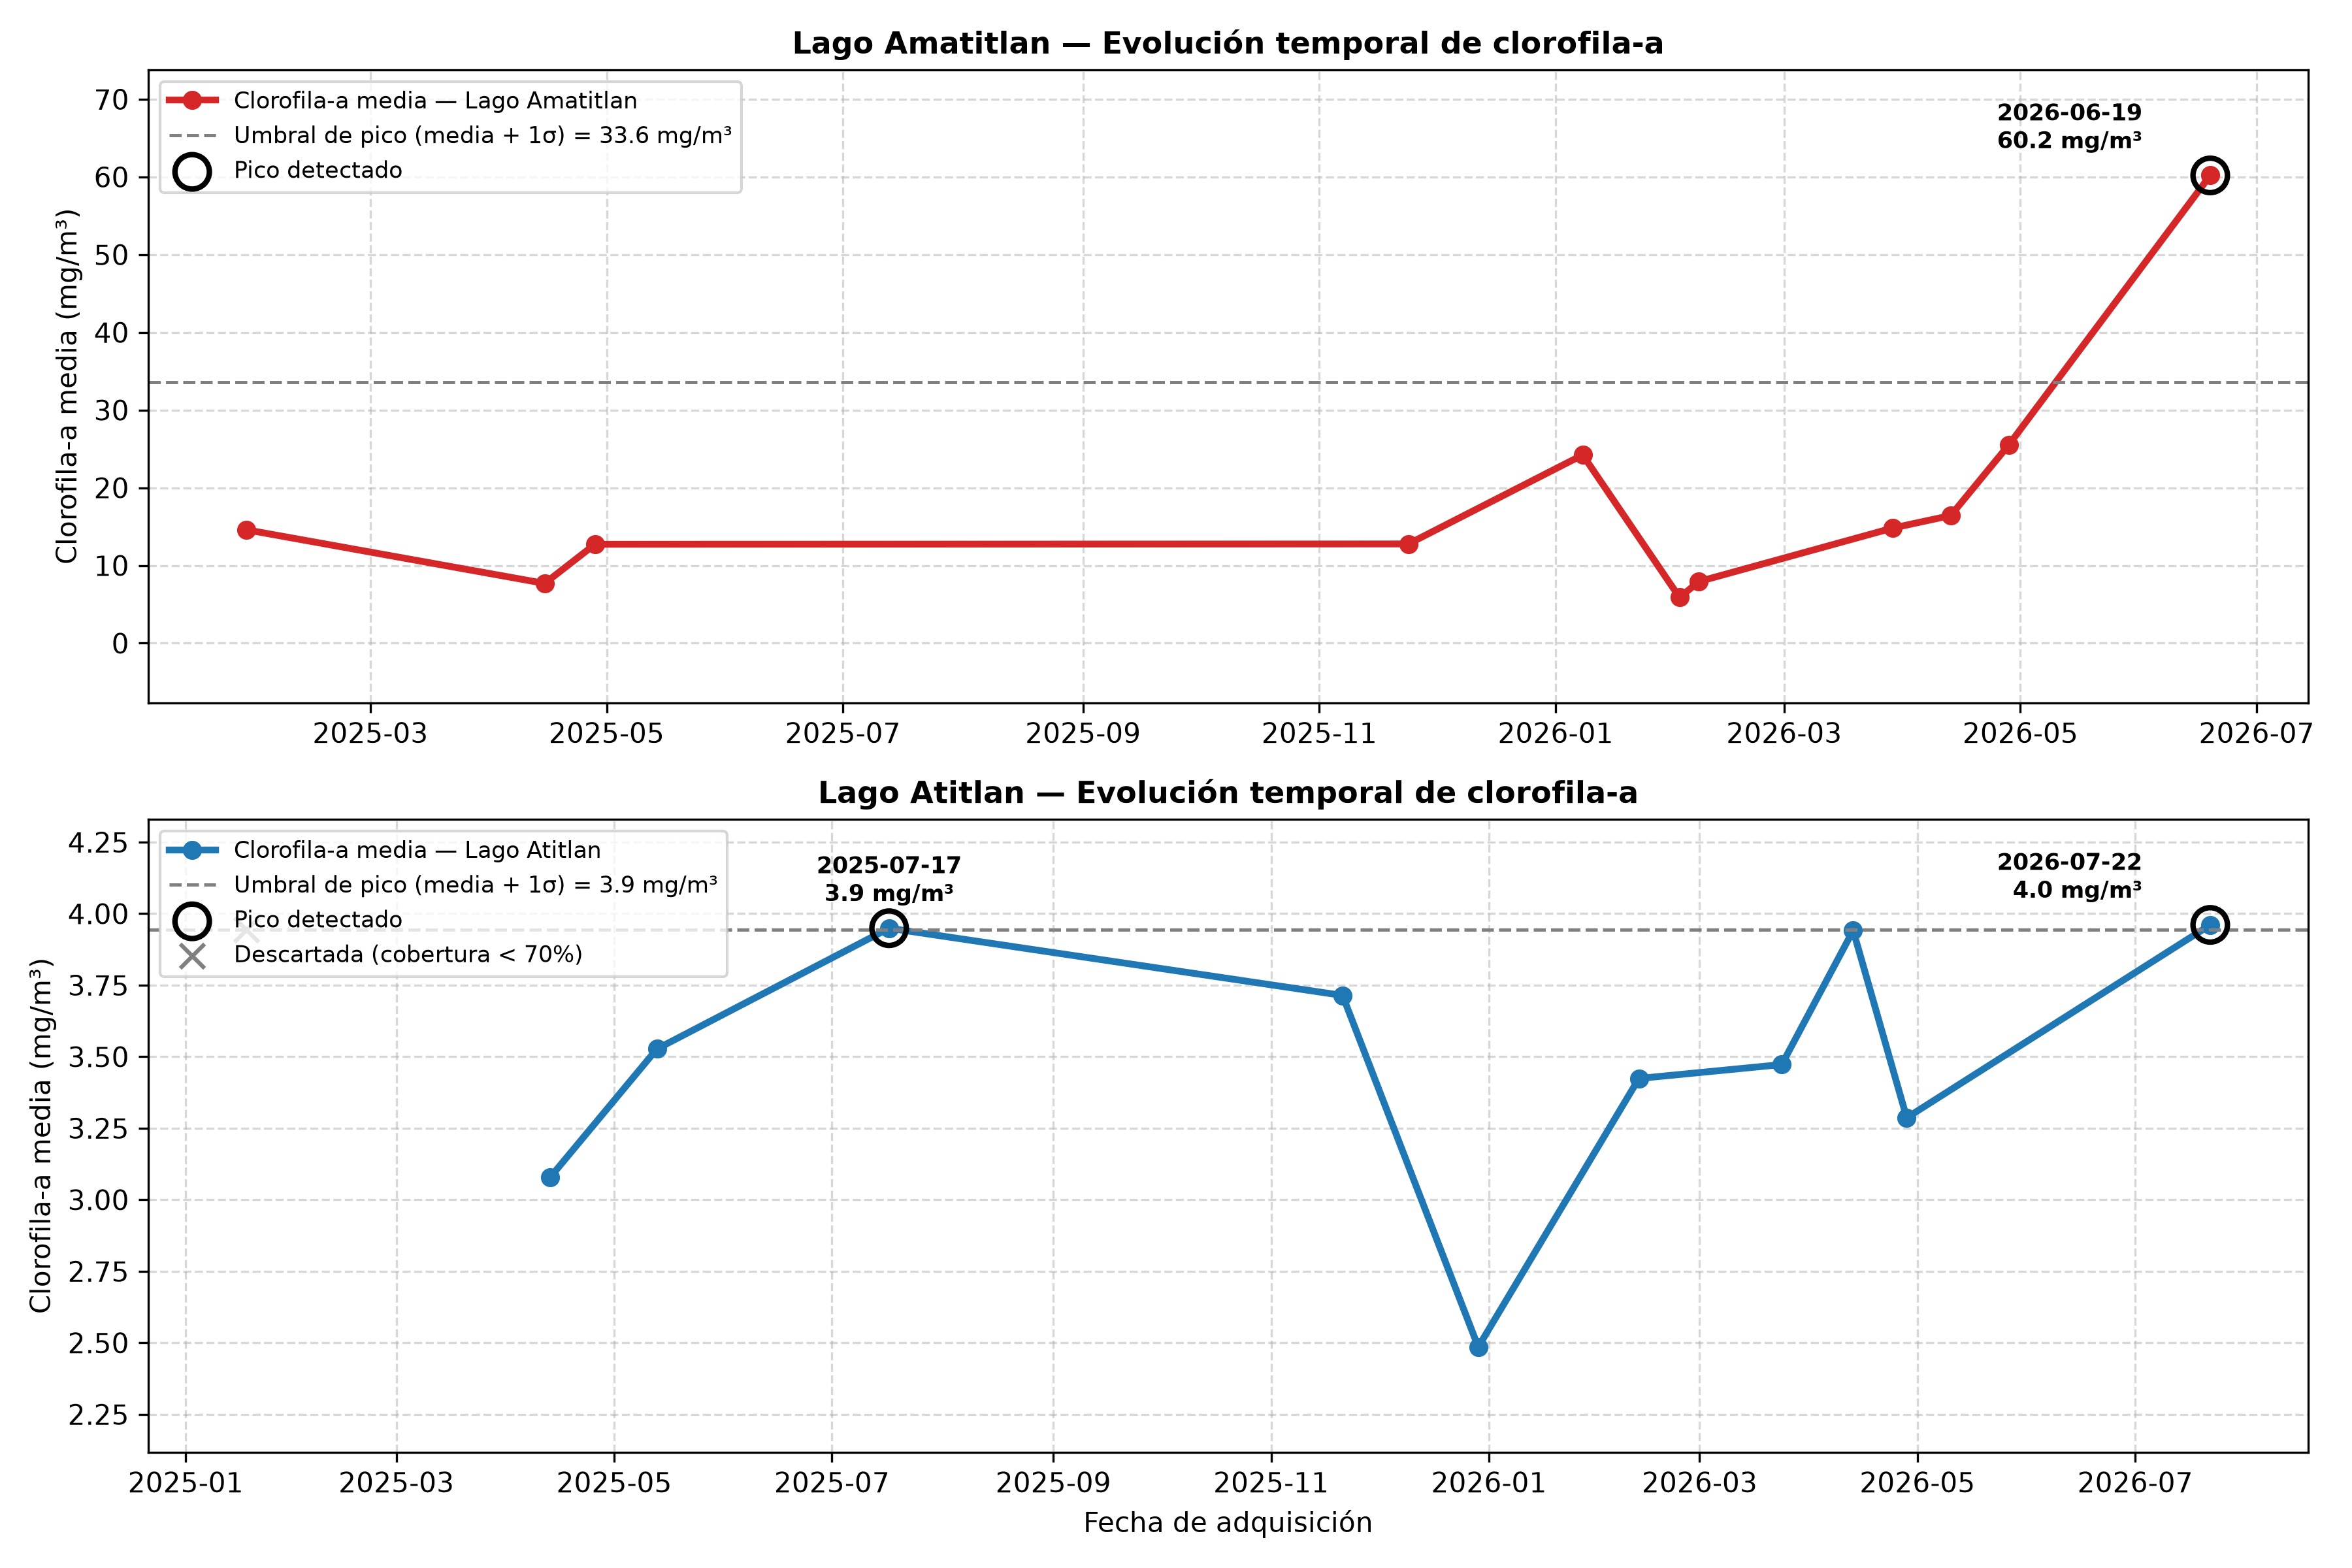
\includegraphics[width=0.92\textwidth]{serie_temporal_picos.png}
    \caption{Evoluci\'on de la clorofila-a media por fecha en Amatitl\'an (arriba) y Atitl\'an (abajo). La l\'inea punteada gris marca el umbral de pico (media + una desviaci\'on est\'andar de cada lago); los c\'irculos negros marcan las fechas identificadas como pico.}
    \label{fig:serie_temporal}
\end{figure}

\textbf{Amatitl\'an} muestra una media de 18.4 mg/m\textsuperscript{3} con una desviaci\'on de 15.2, es decir, una variaci\'on muy grande entre fechas: el valor m\'as bajo del per\'iodo (5.9 mg/m\textsuperscript{3}, en 2026-02-02) es diez veces menor que el m\'as alto (60.2 mg/m\textsuperscript{3}, en 2026-06-19). El nivel de fondo nunca baja de esos 5.9 mg/m\textsuperscript{3}: no existe, en las 11 fechas analizadas, ninguna que pueda llamarse ``lago limpio''. El criterio de media m\'as una desviaci\'on marca una \'unica fecha cr\'itica, 2026-06-19, en la que adem\'as el 76.6\,\% de la superficie del lago (unos 10.6 de sus 13.8 km\textsuperscript{2}) super\'o el umbral de 30 mg/m\textsuperscript{3} que en este informe se usa como referencia de floraci\'on densa.

\textbf{Atitl\'an}, en cambio, se mueve en una banda mucho m\'as angosta: 3.48 $\pm$ 0.46 mg/m\textsuperscript{3}, entre 2.49 y 3.96 mg/m\textsuperscript{3} a lo largo de las 10 fechas confiables, una variaci\'on de apenas 1.6 veces. En promedio, solo el 0.22\,\% de su superficie supera los 30 mg/m\textsuperscript{3}. El criterio estad\'istico marca dos fechas (2025-07-17 y 2026-07-22) como ``pico'', pero superan el umbral por cent\'esimas de mg/m\textsuperscript{3}: son fluctuaciones dentro del ruido normal de la medici\'on, no eventos de floraci\'on real a escala de lago.

La Figura~\ref{fig:serie_log} presenta la misma informaci\'on en escala logar\'itmica (para poder comparar ambos lagos en un mismo gr\'afico pese a la gran diferencia de magnitud) junto con el porcentaje de superficie de cada lago que supera el umbral de floraci\'on densa en cada fecha.

\begin{figure}[H]
    \centering
    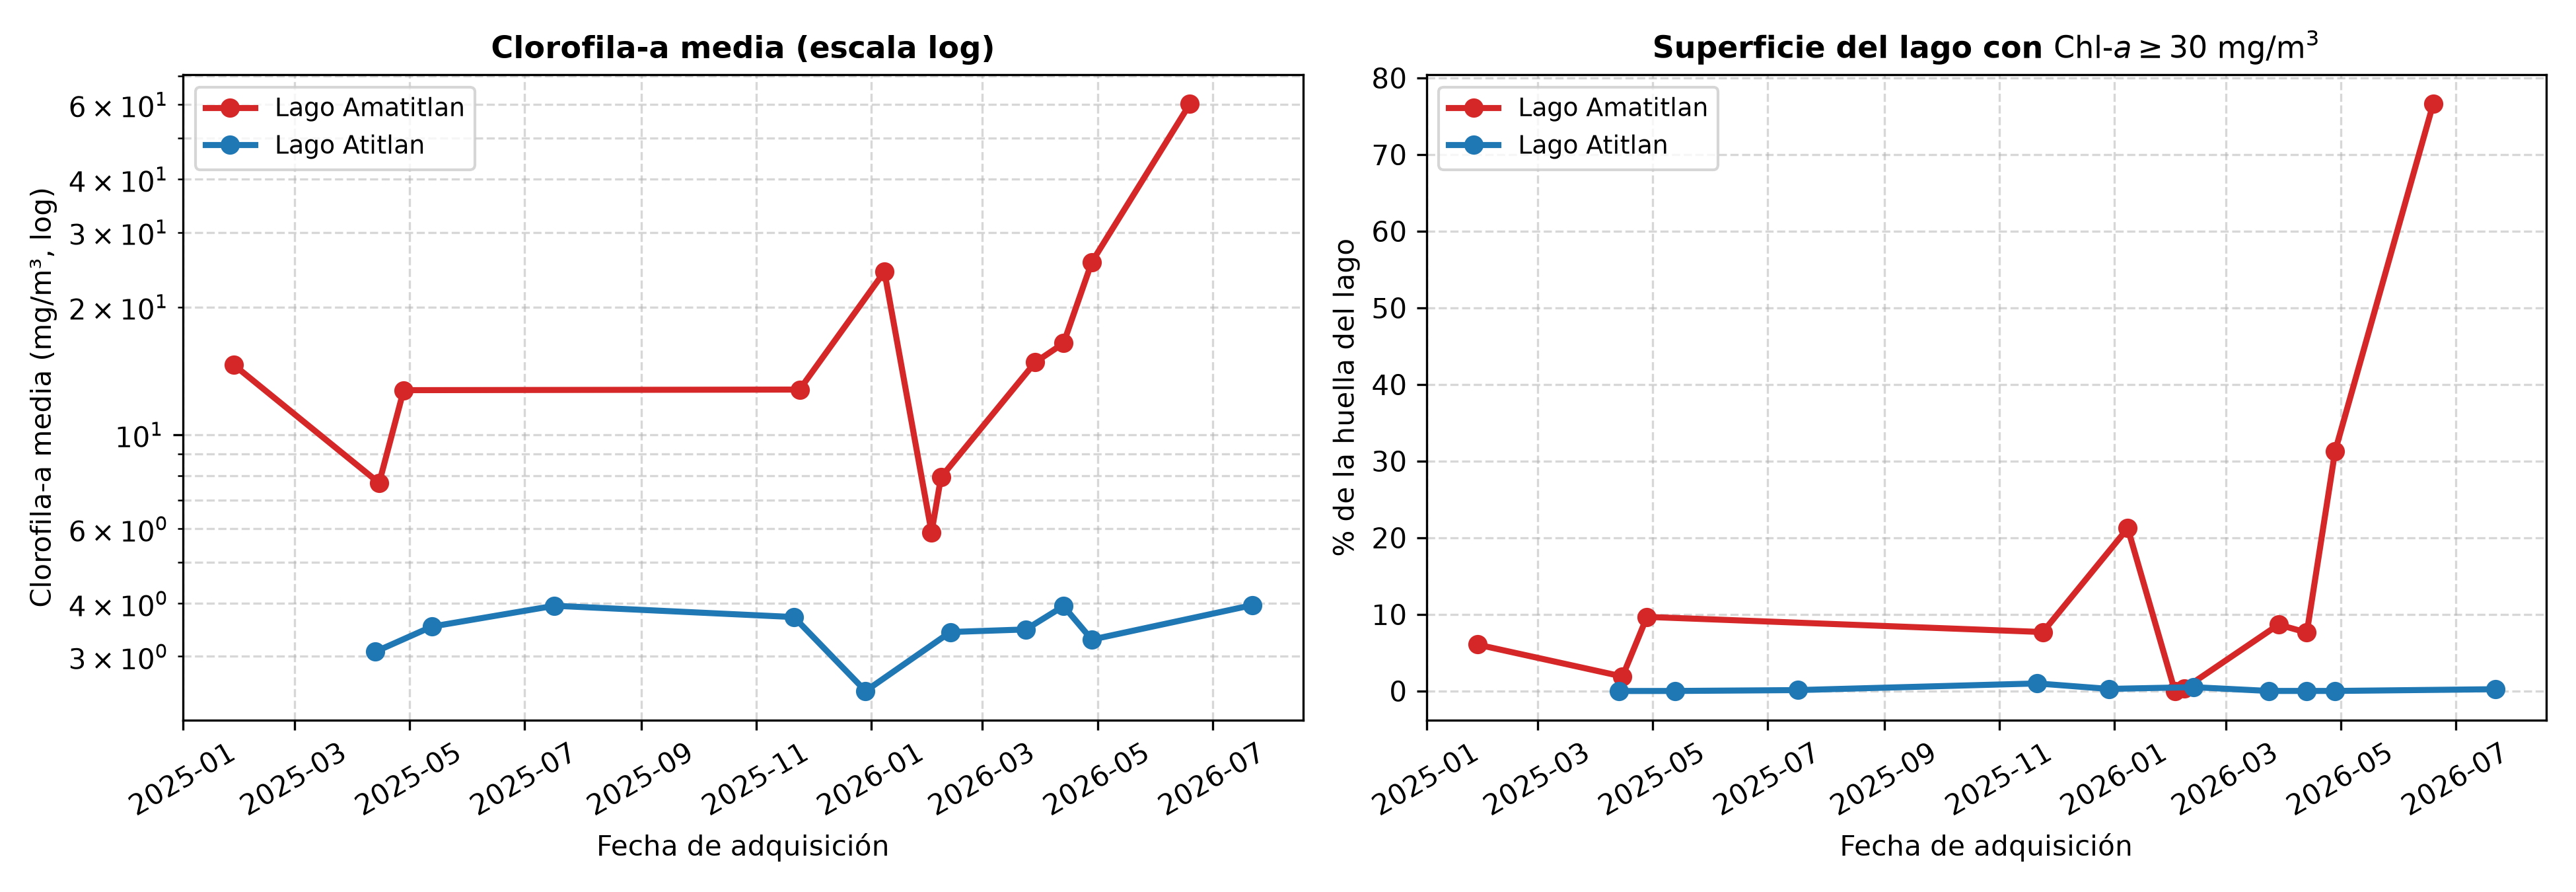
\includegraphics[width=0.95\textwidth]{serie_log_area_alta.png}
    \caption{Izquierda: clorofila-a media por fecha en escala logar\'itmica, comparando ambos lagos en el mismo eje. Derecha: porcentaje de la huella de cada lago que super\'o los 30 mg/m\textsuperscript{3} en cada fecha.}
    \label{fig:serie_log}
\end{figure}

\subsection{¿Qu\'e tipo de floraci\'on es cada pico?}

Comparar la mediana con el promedio de cada fecha ayuda a distinguir dos tipos de evento: cuando ambos valores son parecidos, la floraci\'on sube de forma pareja en todo el lago; cuando el promedio es mucho mayor que la mediana, unas pocas zonas concentradas est\'an ``jalando'' el promedio hacia arriba mientras el resto del lago sigue relativamente limpio.

En Amatitl\'an, la fecha de mayor floraci\'on (2026-06-19) tiene una raz\'on mediana/promedio de 0.98: es una floraci\'on de lago completo, pr\'acticamente uniforme. En cambio, fechas como 2026-04-28 (raz\'on 0.41) muestran manchas localizadas, t\'ipicamente cerca de los puntos donde entra agua de alg\'un afluente contaminado; esa misma fecha es, adem\'as, la que registr\'o m\'as vegetaci\'on o nata flotante detectada (3.1\,\% de la superficie).

% ======================================================================
\section{An\'alisis espacial}
% ======================================================================

Adem\'as de la evoluci\'on temporal, interesa saber \emph{d\'onde dentro de cada lago} se concentra la cianobacteria. Para esto se construy\'o un mapa interactivo (con la librer\'ia \texttt{folium}) que permite navegar libremente sobre ambos lagos y consultar, con un clic, las estad\'isticas de la fecha de mayor floraci\'on de cada uno; ese mapa se entrega junto con el c\'odigo del proyecto porque su naturaleza interactiva no se puede representar en un documento est\'atico como este. En su lugar, la Figura~\ref{fig:cuadricula_amatitlan} y la Figura~\ref{fig:cuadricula_atitlan} muestran una cuadr\'icula comparativa con la clorofila-a de las 11 fechas de cada lago, una junto a otra, con borde rojo en las fechas identificadas como pico.

\begin{figure}[H]
    \centering
    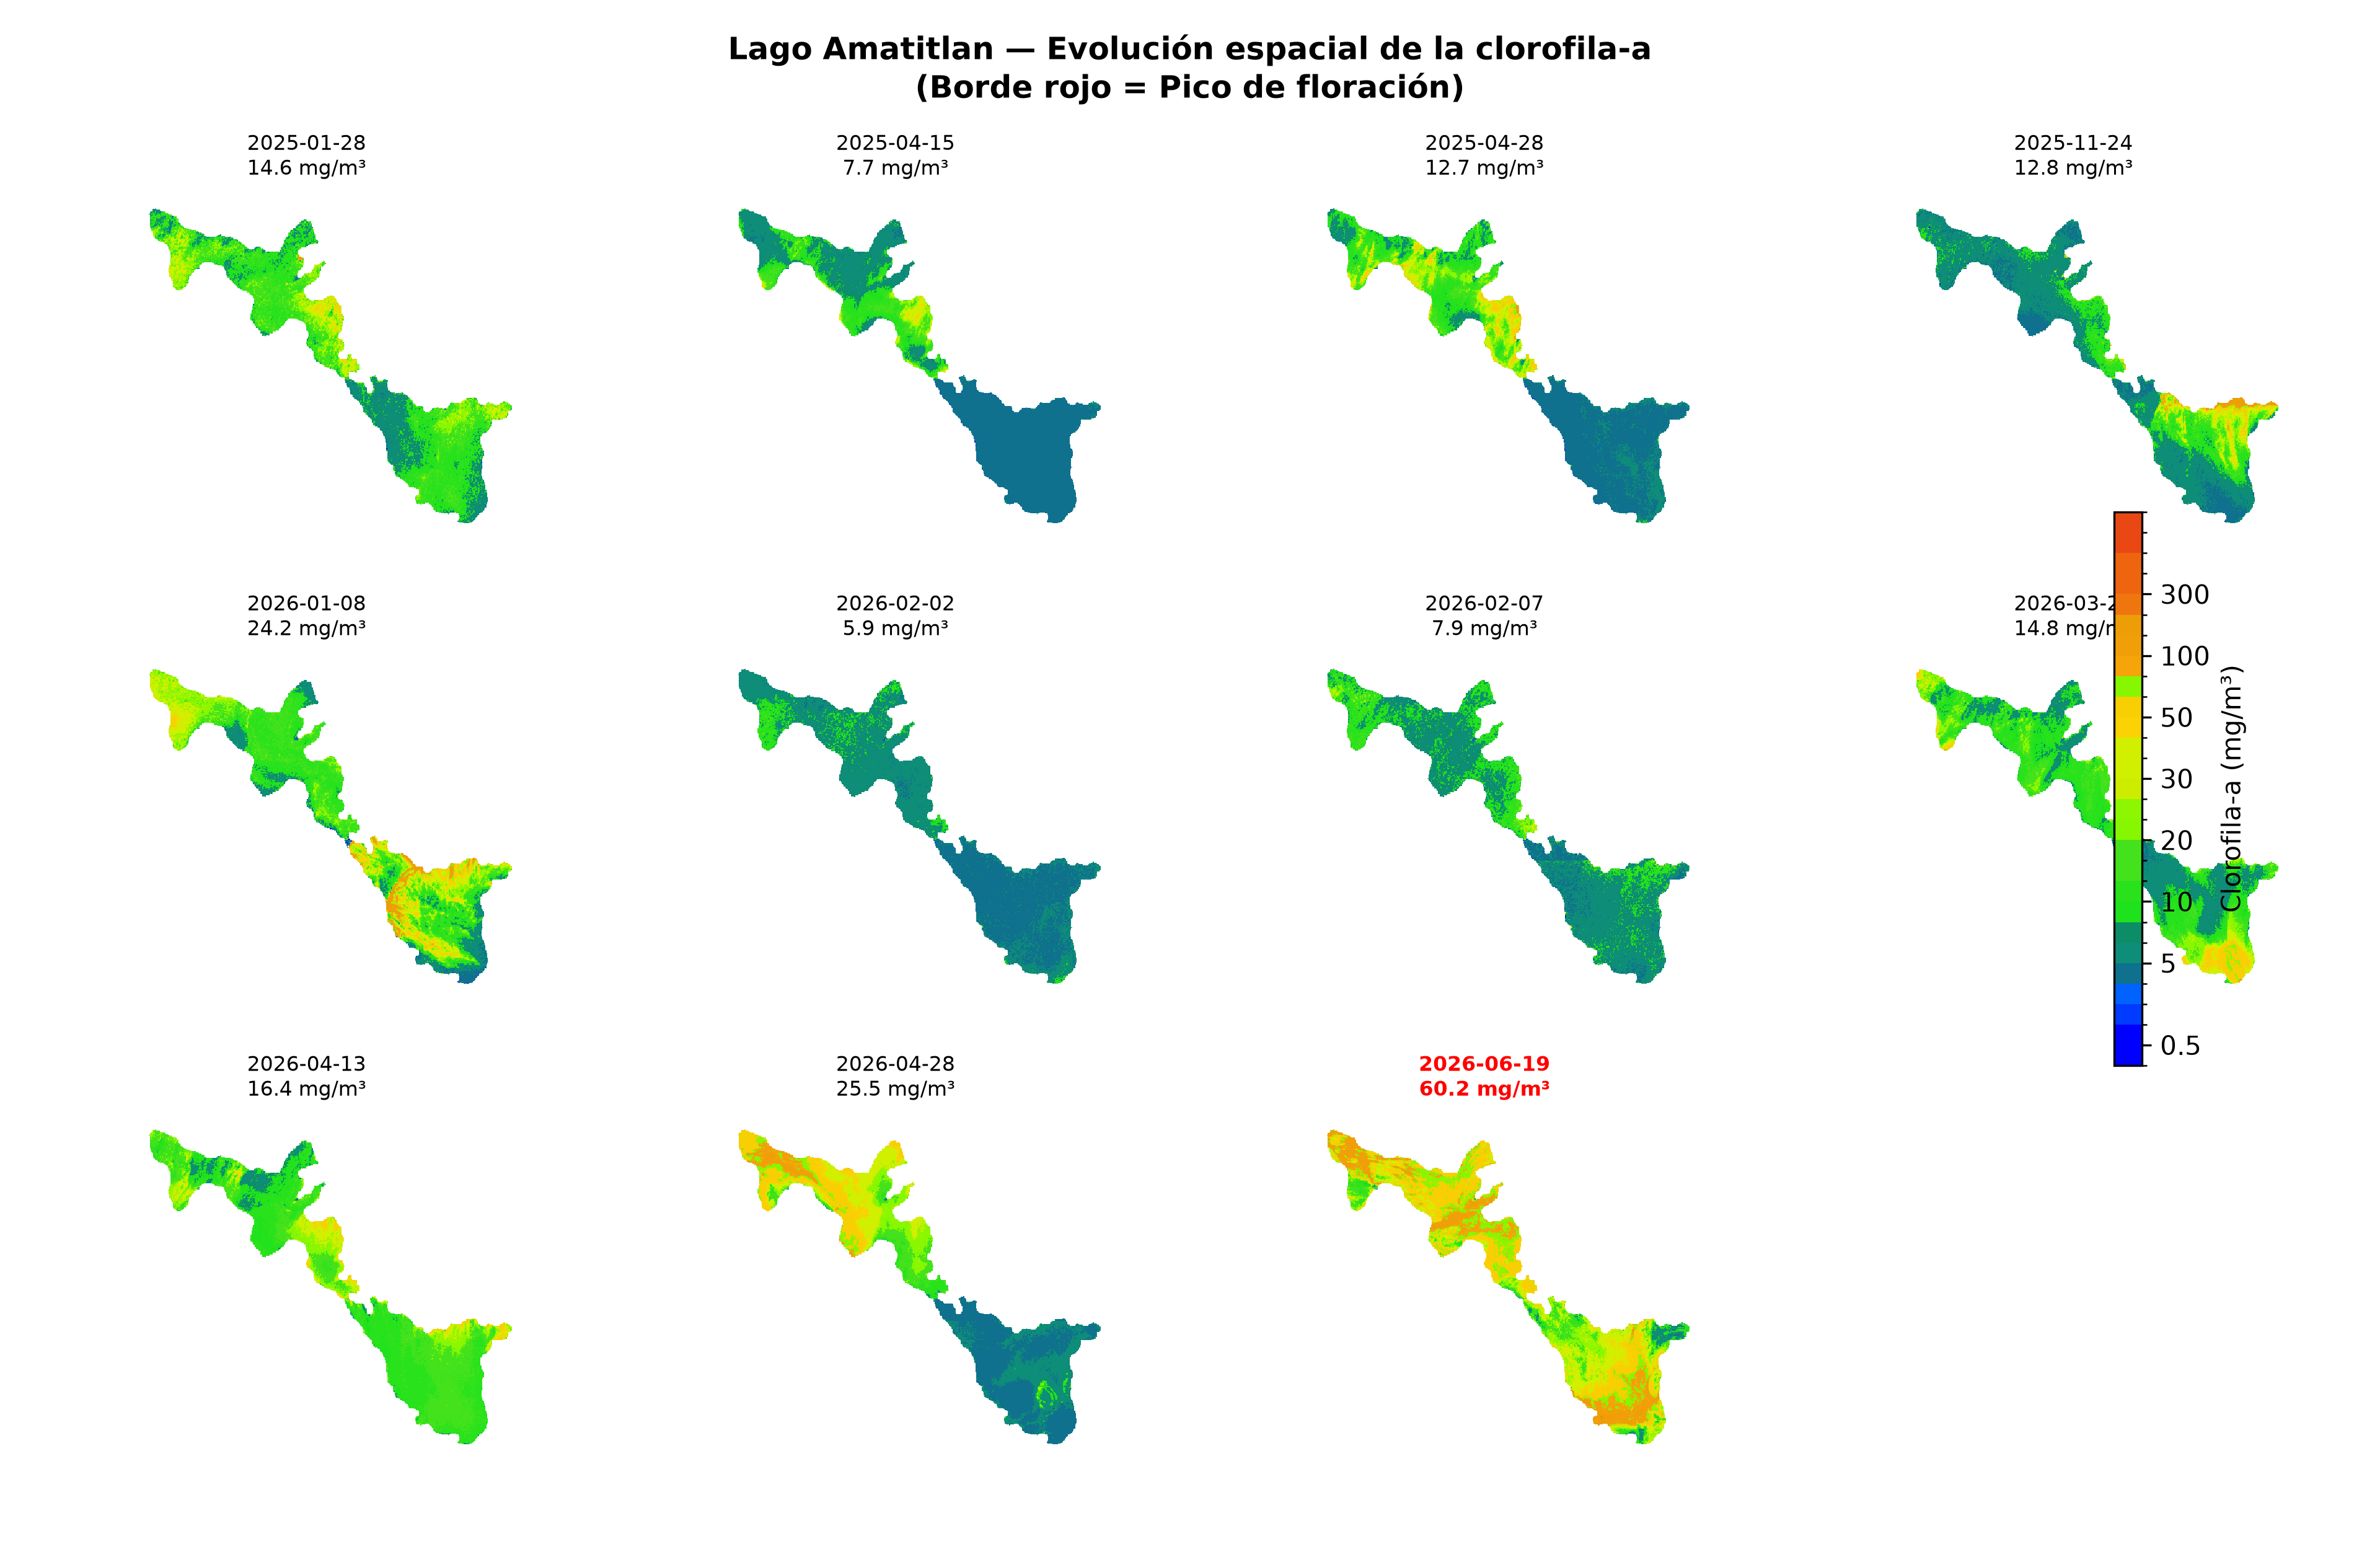
\includegraphics[width=0.92\textwidth]{cuadricula_amatitlan.png}
    \caption{Evoluci\'on espacial de la clorofila-a en Amatitl\'an a lo largo de las 11 fechas analizadas. El borde rojo marca la fecha identificada como pico de floraci\'on.}
    \label{fig:cuadricula_amatitlan}
\end{figure}

\begin{figure}[H]
    \centering
    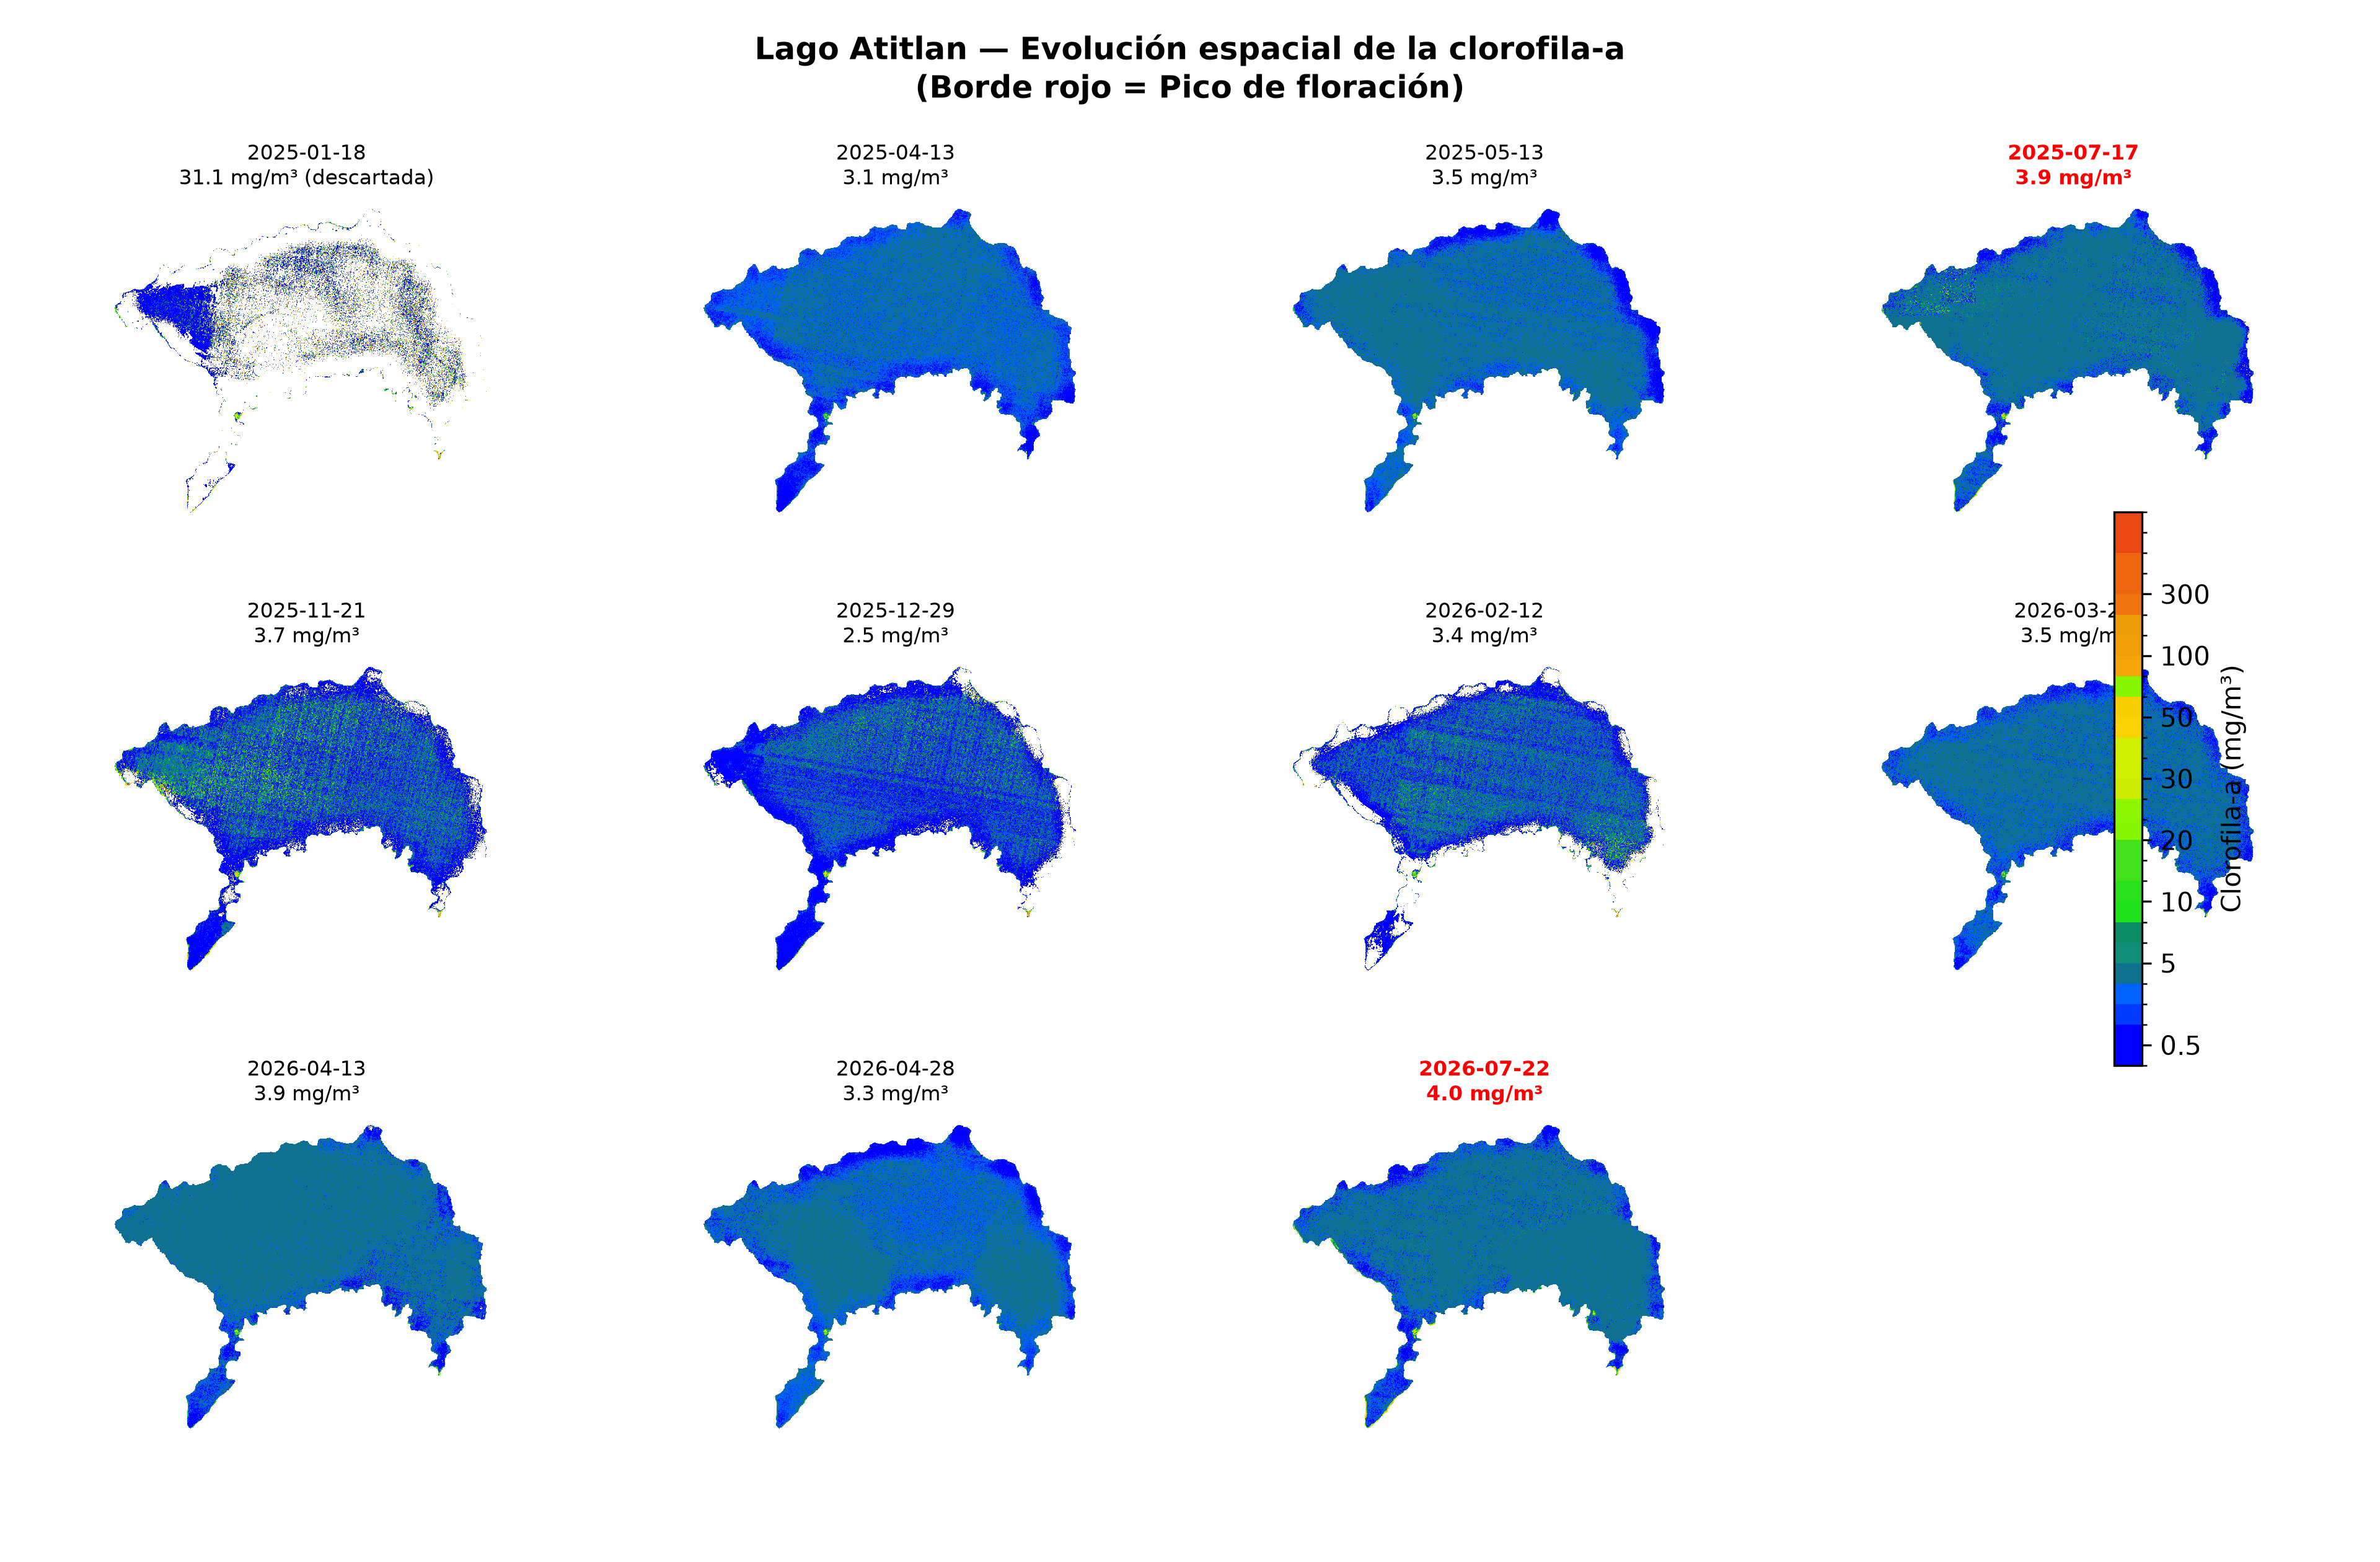
\includegraphics[width=0.92\textwidth]{cuadricula_atitlan.png}
    \caption{Evoluci\'on espacial de la clorofila-a en Atitl\'an a lo largo de las 11 fechas analizadas.}
    \label{fig:cuadricula_atitlan}
\end{figure}

\textbf{En Amatitl\'an}, el foco de mayor concentraci\'on se repite de forma sistem\'atica en la zona noreste del lago, junto a la desembocadura del \textbf{r\'io Villalobos}, el principal receptor de aguas residuales del \'area metropolitana de la Ciudad de Guatemala. En la fecha de floraci\'on total (2026-06-19) la clorofila alta cubre pr\'acticamente todo el espejo de agua; en fechas de floraci\'on en parches (por ejemplo 2026-04-28) las manchas de mayor concentraci\'on aparecen junto a las entradas de afluentes.

\textbf{En Atitl\'an}, la escala de colores es predominantemente azul en la gran mayor\'ia del lago (menos de 5 mg/m\textsuperscript{3}), pero aparecen focos intensos y muy localizados en las bah\'ias de \textbf{Santiago Atitl\'an}, \textbf{San Pedro La Laguna} y \textbf{Panajachel}. En algunas fechas, esos focos alcanzan el tope de la escala del propio script (500 mg/m\textsuperscript{3}) en unos pocos p\'ixeles, mientras el resto del lago permanece limpio. El gran volumen de agua de la caldera vuelc\'anica diluye r\'apidamente lo que llega desde esas bah\'ias, por lo que el promedio de todo el lago no refleja estos eventos locales; de ah\'i la importancia de mirar el mapa y no solo el promedio.

% ======================================================================
\section{Relaci\'on entre la clorofila-a y los \'indices NDVI/NDWI}
% ======================================================================

Se analiz\'o si existe una relaci\'on estad\'istica entre la clorofila-a estimada y los \'indices NDVI y NDWI, calculados sobre la huella de cada lago en cada fecha confiable. La hip\'otesis es que, cuando aumenta la biomasa de algas, el NDVI deber\'ia subir (porque las algas reflejan m\'as infrarrojo cercano, igual que la vegetaci\'on terrestre) y el NDWI deber\'ia bajar (porque el agua cargada de pigmentos absorbe la luz de forma distinta al agua limpia).

\begin{figure}[H]
    \centering
    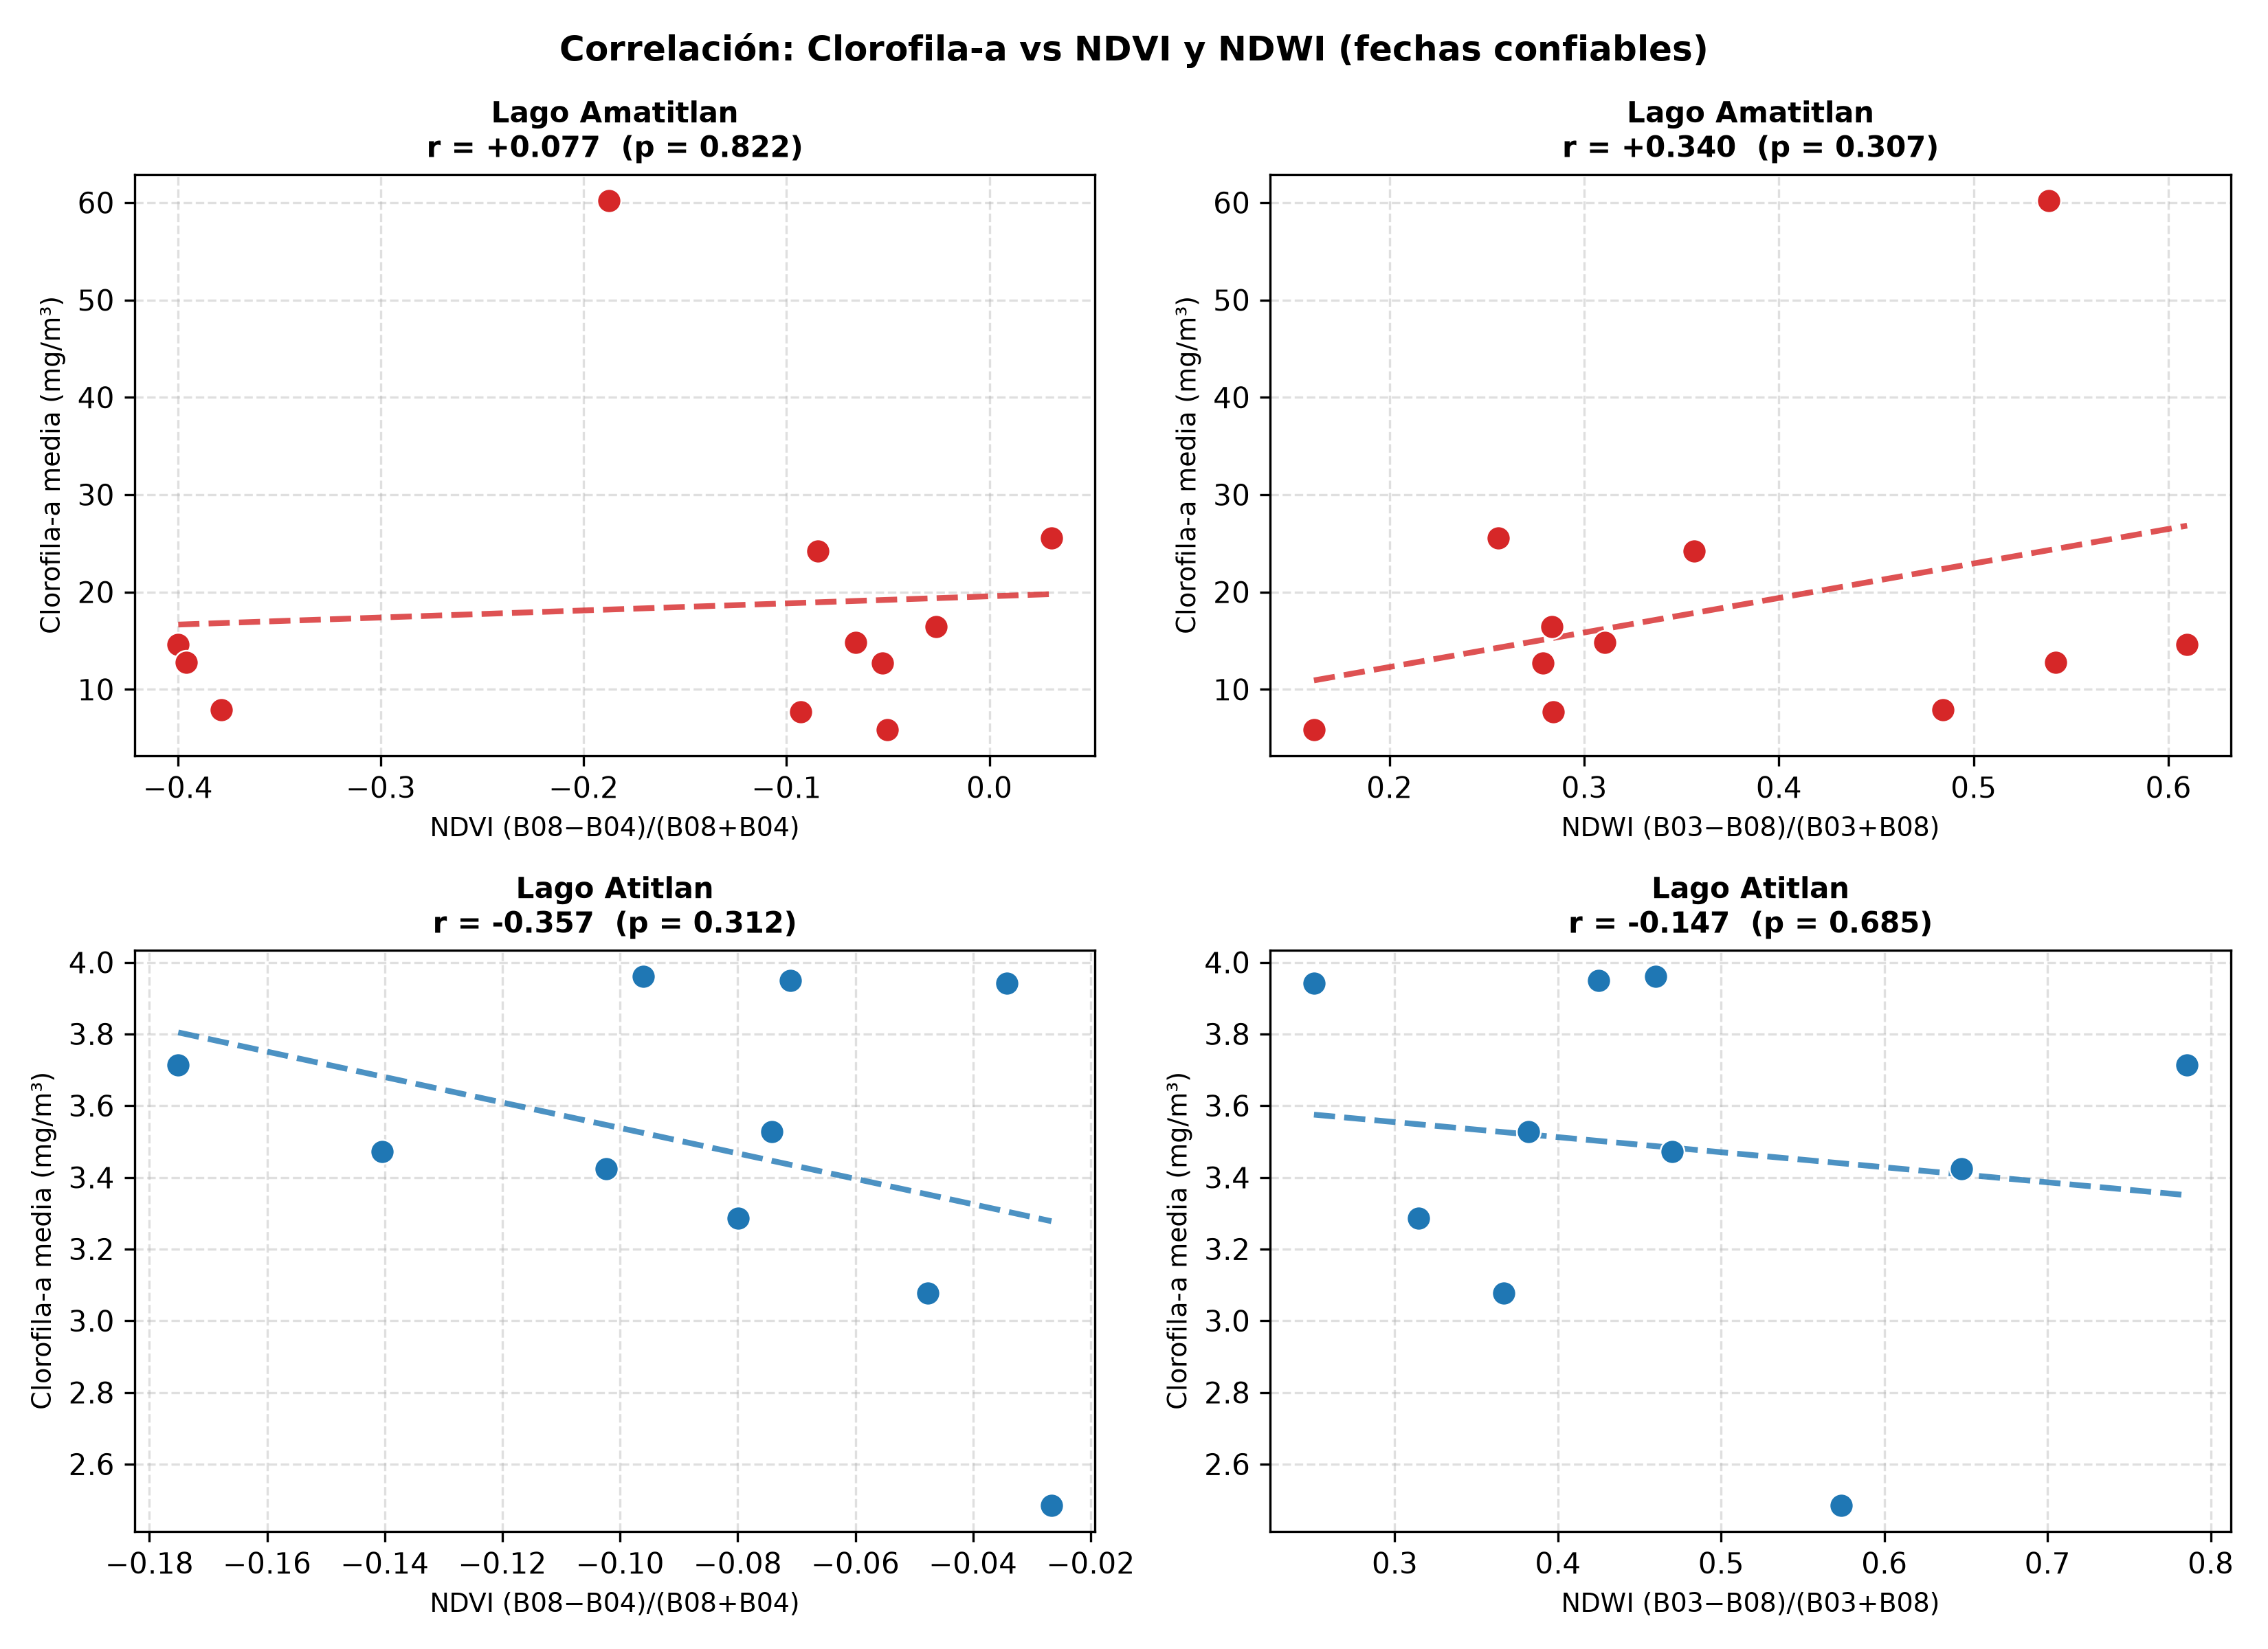
\includegraphics[width=0.85\textwidth]{correlacion_ndvi_ndwi.png}
    \caption{Correlaci\'on entre la clorofila-a media por fecha y los \'indices NDVI (izquierda) y NDWI (derecha), para Amatitl\'an (arriba) y Atitl\'an (abajo). \emph{r} es el coeficiente de correlaci\'on de Pearson y \emph{p} indica si esa correlaci\'on es estad\'isticamente significativa.}
    \label{fig:correlacion}
\end{figure}

\begin{table}[H]
\centering
\caption{Resumen de las correlaciones entre clorofila-a y los \'indices espectrales.}
\label{tab:correlaciones}
\begin{tabular}{lcccc}
\toprule
Lago & $r$ (NDVI) & $p$ (NDVI) & $r$ (NDWI) & $p$ (NDWI) \\
\midrule
Amatitl\'an & +0.077 & 0.822 & +0.340 & 0.307 \\
Atitl\'an   & --0.357 & 0.312 & --0.147 & 0.685 \\
\bottomrule
\end{tabular}
\end{table}

En ninguno de los dos lagos la correlaci\'on result\'o estad\'isticamente significativa ($p > 0.05$ en los cuatro casos), lo cual, m\'as que un resultado negativo, tiene una explicaci\'on razonable: con solo 10 u 11 fechas por lago, y en el caso de Atitl\'an con una variaci\'on de clorofila-a muy peque\~na entre fechas (desviaci\'on de apenas 0.46 mg/m\textsuperscript{3}), el ruido natural de la medici\'on satelital pesa m\'as que cualquier se\~nal real. Es probable que, a escala de p\'ixel individual dentro de las bah\'ias donde s\'i hay floraciones locales en Atitl\'an, la relaci\'on entre estos \'indices sea m\'as clara; ese an\'alisis a nivel de p\'ixel queda como l\'inea de trabajo futura. En Amatitl\'an, aunque tampoco alcanza significancia estad\'istica con solo 11 puntos, el signo de las correlaciones (positivo con NDVI, positivo con NDWI en este caso particular) es consistente con la direcci\'on esperada del fen\'omeno.

% ======================================================================
\section{Comparaci\'on entre los dos lagos}
% ======================================================================

\begin{figure}[H]
    \centering
    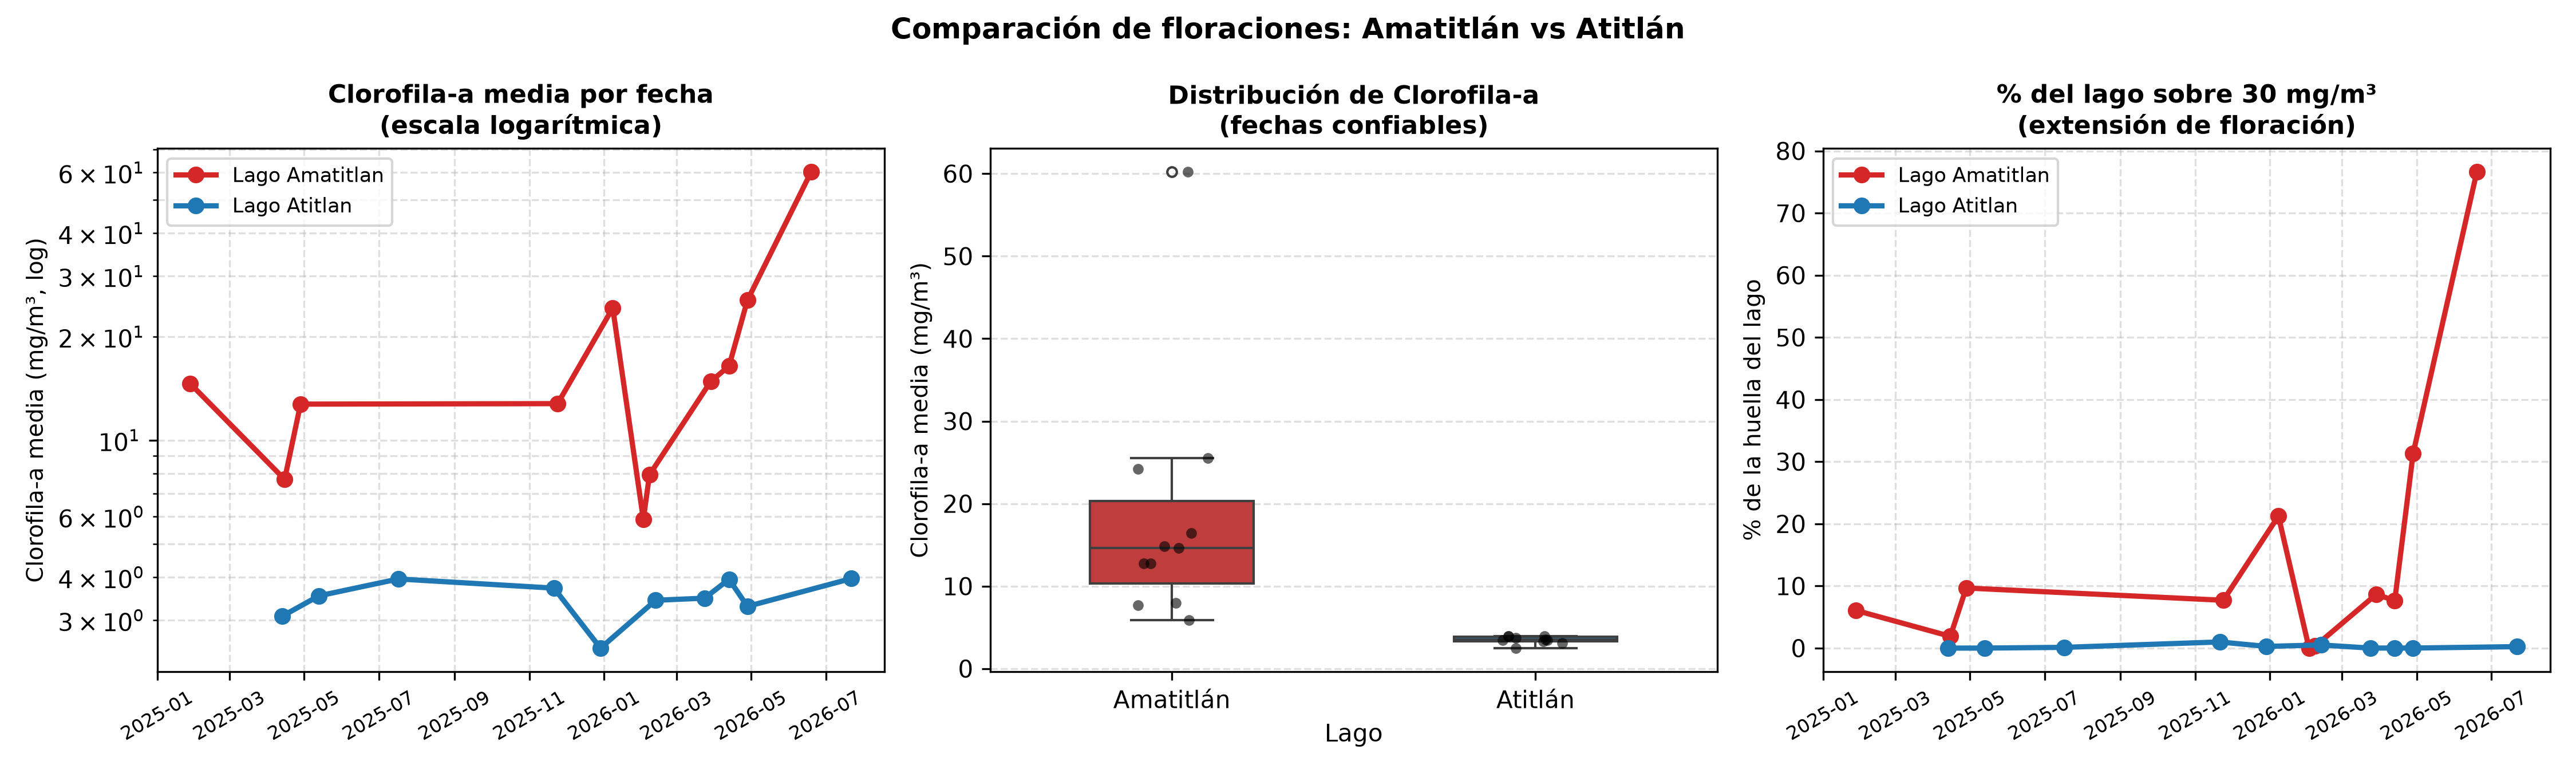
\includegraphics[width=0.95\textwidth]{comparacion_lagos.png}
    \caption{Comparaci\'on directa entre Amatitl\'an y Atitl\'an: serie temporal en escala logar\'itmica (izquierda), distribuci\'on de la clorofila-a media por fecha (centro) y porcentaje de superficie sobre el umbral de floraci\'on densa (derecha).}
    \label{fig:comparacion}
\end{figure}

\begin{table}[H]
\centering
\caption{Indicadores comparativos entre ambos lagos, calculados sobre las fechas confiables del per\'iodo enero 2025 -- julio 2026.}
\label{tab:comparativa}
\begin{tabular}{lcc}
\toprule
Indicador & Amatitl\'an & Atitl\'an \\
\midrule
Clorofila-a media del per\'iodo & 18.4 mg/m\textsuperscript{3} & 3.5 mg/m\textsuperscript{3} \\
M\'aximo registrado (promedio de una fecha) & 60.2 mg/m\textsuperscript{3} & 4.0 mg/m\textsuperscript{3} \\
Superficie sobre 30 mg/m\textsuperscript{3} (promedio) & 15.6\,\% & 0.22\,\% \\
Variaci\'on entre fechas (m\'ax/m\'in) & 10.2$\times$ & 1.6$\times$ \\
Superficie de la huella del lago & 13.8 km\textsuperscript{2} & 120.8 km\textsuperscript{2} \\
N\'umero de picos detectados & 1 & 2 (marginales) \\
\bottomrule
\end{tabular}
\end{table}

La diferencia entre ambos lagos no es de grado, sino de r\'egimen: en promedio, Amatitl\'an tiene 5.3 veces m\'as clorofila-a que Atitl\'an, y su fecha m\'as floreada llega a 15 veces el valor m\'aximo jam\'as observado en Atitl\'an durante el mismo per\'iodo.

Varios factores geogr\'aficos y de uso del suelo ayudan a explicar esta diferencia:

\begin{itemize}
    \item \textbf{Volumen de agua disponible para diluir nutrientes.} Amatitl\'an es un lago somero de unos 33 metros de profundidad media y apenas 13.8 km\textsuperscript{2}; Atitl\'an, formado dentro de una caldera volc\'anica, supera los 300 metros de profundidad en su punto m\'as hondo y tiene casi diez veces la superficie de Amatitl\'an. Un volumen mucho mayor diluye con mayor facilidad los nutrientes que llegan desde la cuenca.
    \item \textbf{Presi\'on urbana e industrial en la cuenca.} Amatitl\'an recibe, a trav\'es del r\'io Villalobos, buena parte del drenaje del \'area metropolitana de la Ciudad de Guatemala, con varios millones de habitantes en su cuenca. Atitl\'an, en cambio, est\'a rodeado principalmente por municipios del altiplano con una poblaci\'on y actividad industrial mucho menores, aunque con presi\'on tur\'istica creciente.
    \item \textbf{Tipo de afluentes.} Mientras Amatitl\'an tiene un afluente principal claramente identificado como fuente de nutrientes, Atitl\'an recibe agua de varios r\'ios menores y de lluvia directa, m\'as distribuidos alrededor del lago.
\end{itemize}

En conjunto, esto sit\'ua a Amatitl\'an en un estado de \textbf{eutrofizaci\'on cr\'onica documentada} (con un evento de floraci\'on que cubri\'o el 76.6\,\% del lago en junio de 2026), mientras que Atitl\'an se mantiene en un estado saludable a nivel de lago completo, con focos locales puntuales en zonas de mayor actividad humana que merecen monitoreo continuo para evitar que se agraven.

% ======================================================================
\section{An\'alisis exploratorio adicional}
% ======================================================================

\subsection{Extensi\'on espacial de la floraci\'on por fecha}

M\'as all\'a del promedio, interesa saber qu\'e porcentaje del lago estuvo, en cada fecha, por encima del umbral de floraci\'on densa (30 mg/m\textsuperscript{3}).

\begin{figure}[H]
    \centering
    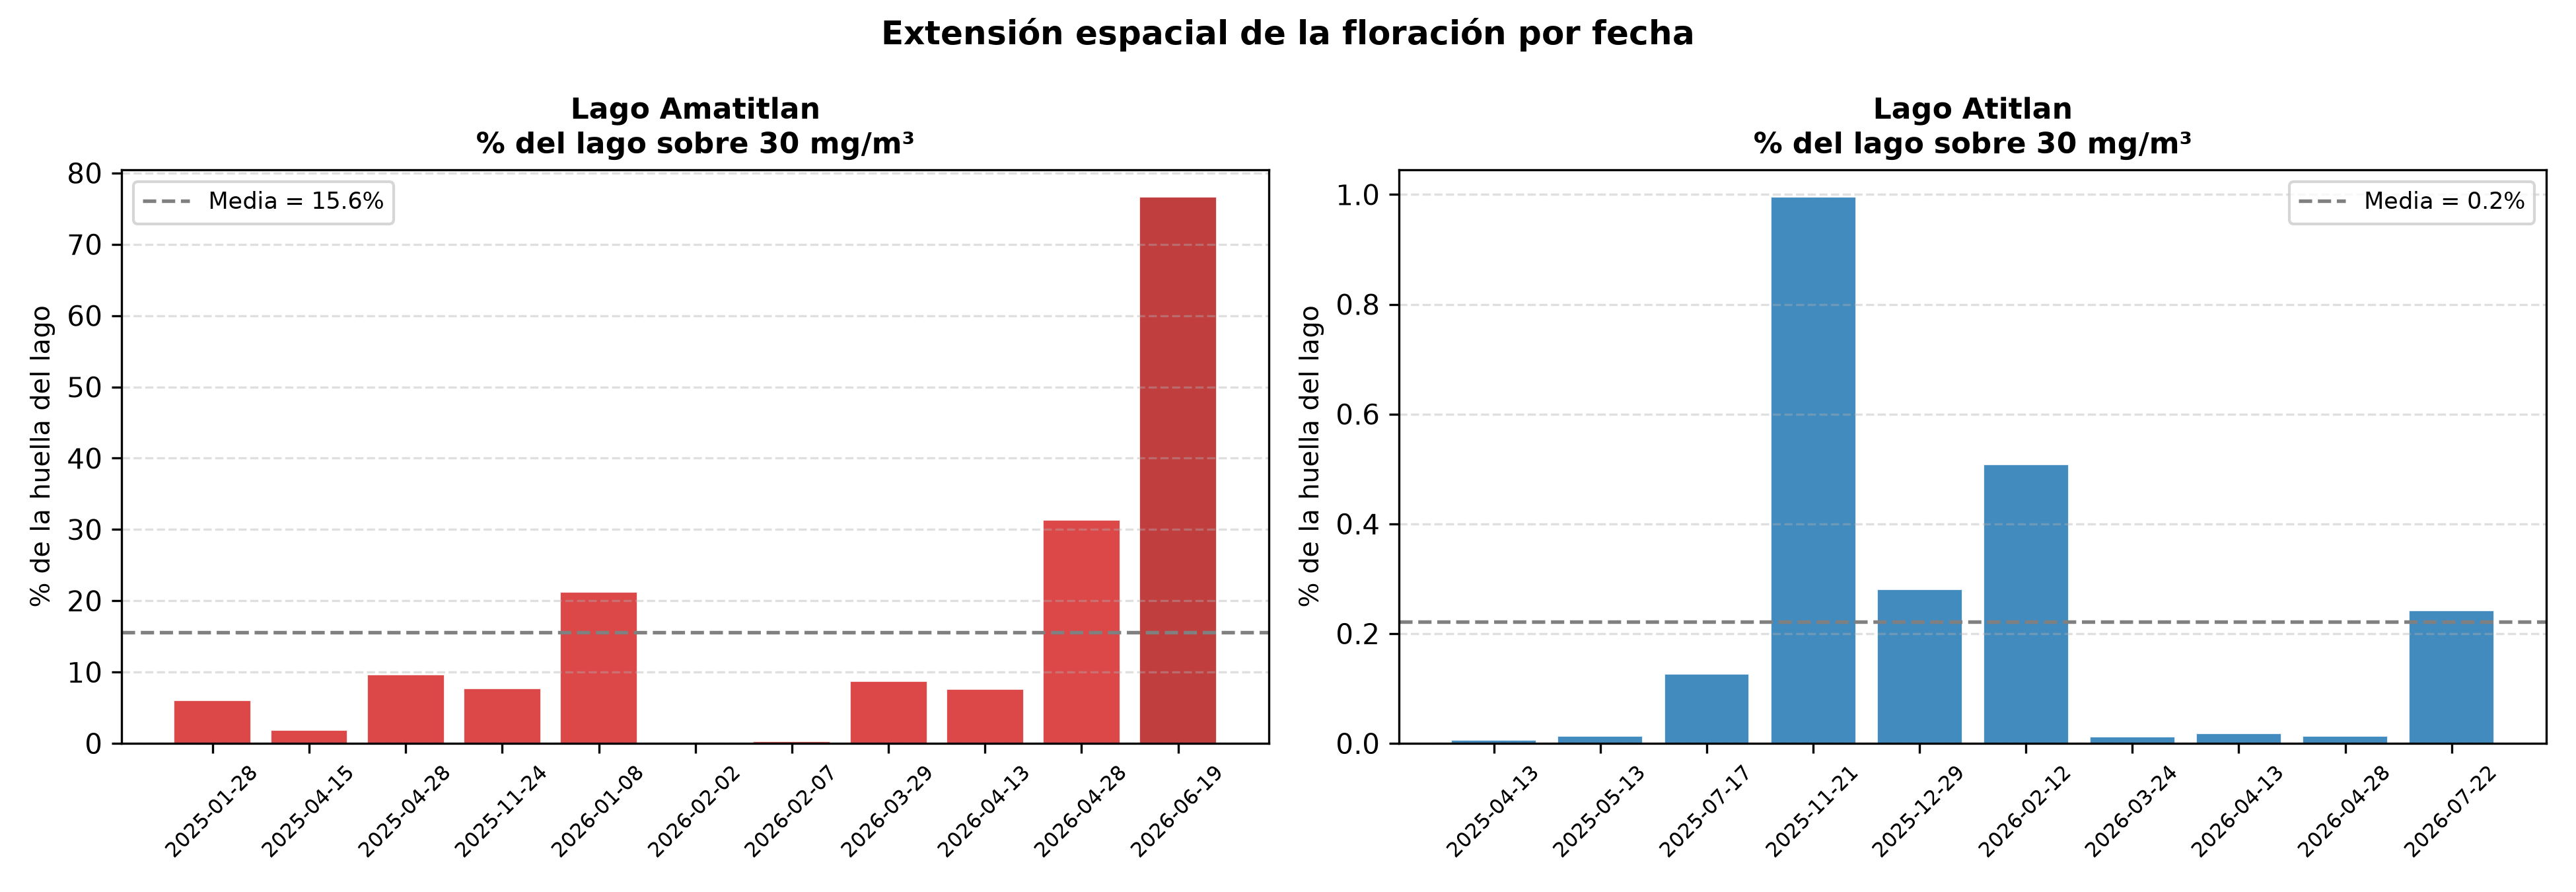
\includegraphics[width=0.92\textwidth]{extension_espacial.png}
    \caption{Porcentaje de la superficie de cada lago por encima de 30 mg/m\textsuperscript{3} de clorofila-a, fecha por fecha.}
    \label{fig:extension}
\end{figure}

El contraste es claro: en 2026-06-19, Amatitl\'an lleg\'o a tener el 76.6\,\% de su espejo de agua por encima del umbral, es decir, una floraci\'on de lago completo y no un evento localizado. En Atitl\'an, ninguna fecha del per\'iodo super\'o el 1.5\,\% de su superficie sobre ese mismo umbral: los valores altos que existen corresponden siempre a focos puntuales, nunca a un evento generalizado.

\subsection{Zonas persistentes de acumulaci\'on}

Promediando la clorofila-a p\'ixel por p\'ixel a lo largo de las 11 fechas de cada lago, es posible identificar qu\'e zonas concentran valores altos de forma recurrente, m\'as all\'a de una sola fecha puntual.

\begin{figure}[H]
    \centering
    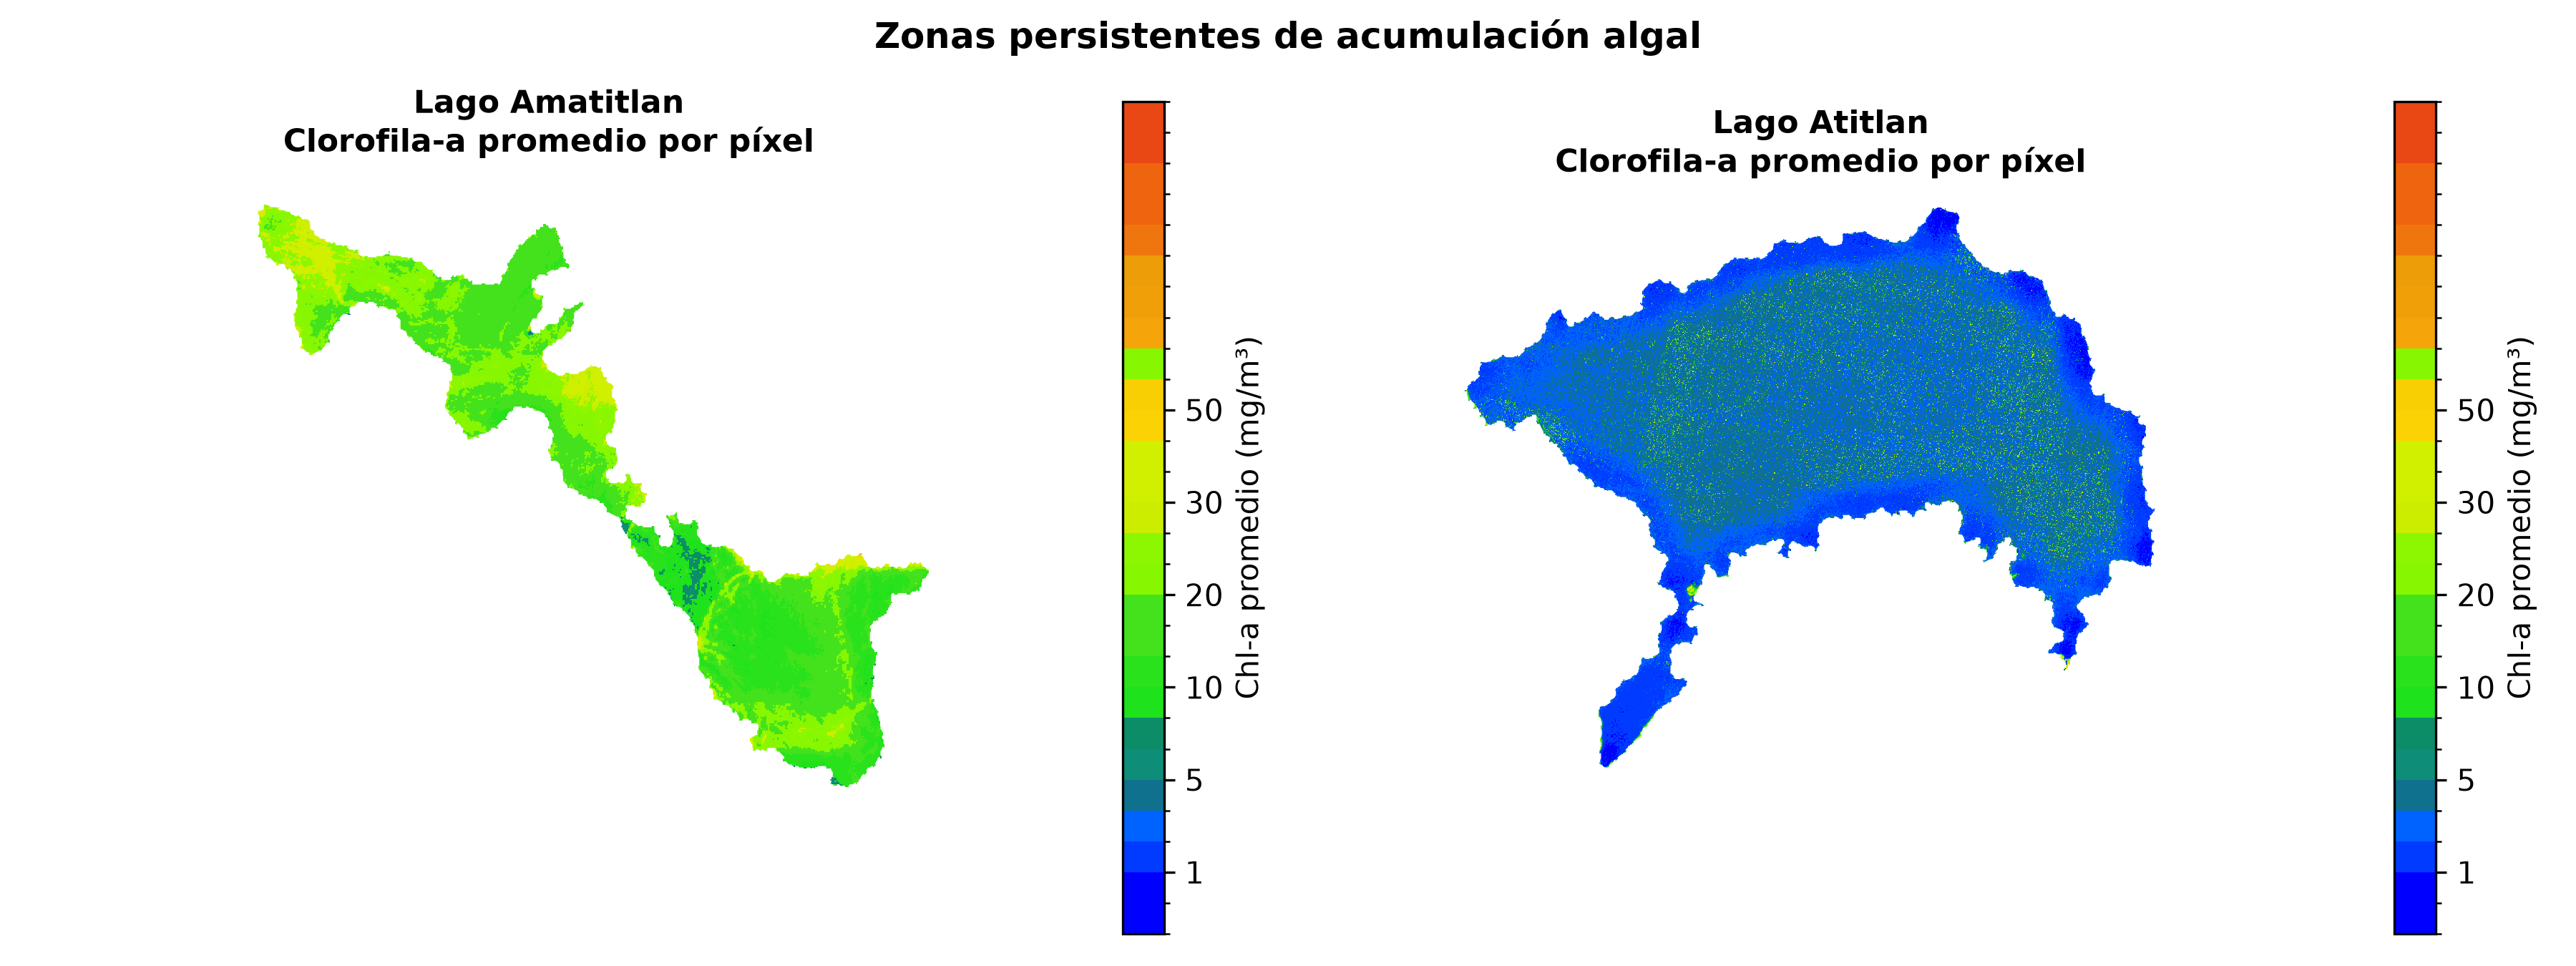
\includegraphics[width=0.92\textwidth]{zonas_persistentes.png}
    \caption{Clorofila-a promedio por p\'ixel a lo largo de las 11 fechas, para Amatitl\'an (izquierda) y Atitl\'an (derecha). Los tonos amarillo/naranja marcan zonas de acumulaci\'on persistente.}
    \label{fig:zonas_persistentes}
\end{figure}

En \textbf{Amatitl\'an}, el sector norte y noreste del lago concentra los valores m\'as altos de manera recurrente, en l\'inea con la entrada del r\'io Villalobos identificada anteriormente. En \textbf{Atitl\'an}, los focos persistentes corresponden justamente a las bah\'ias con mayor actividad humana mencionadas antes (Santiago Atitl\'an, San Pedro La Laguna, Panajachel), mientras que el centro del lago se mantiene limpio de forma consistente en todas las fechas.

\subsection{C\'omo se distribuyen los valores dentro de cada lago}

\begin{figure}[H]
    \centering
    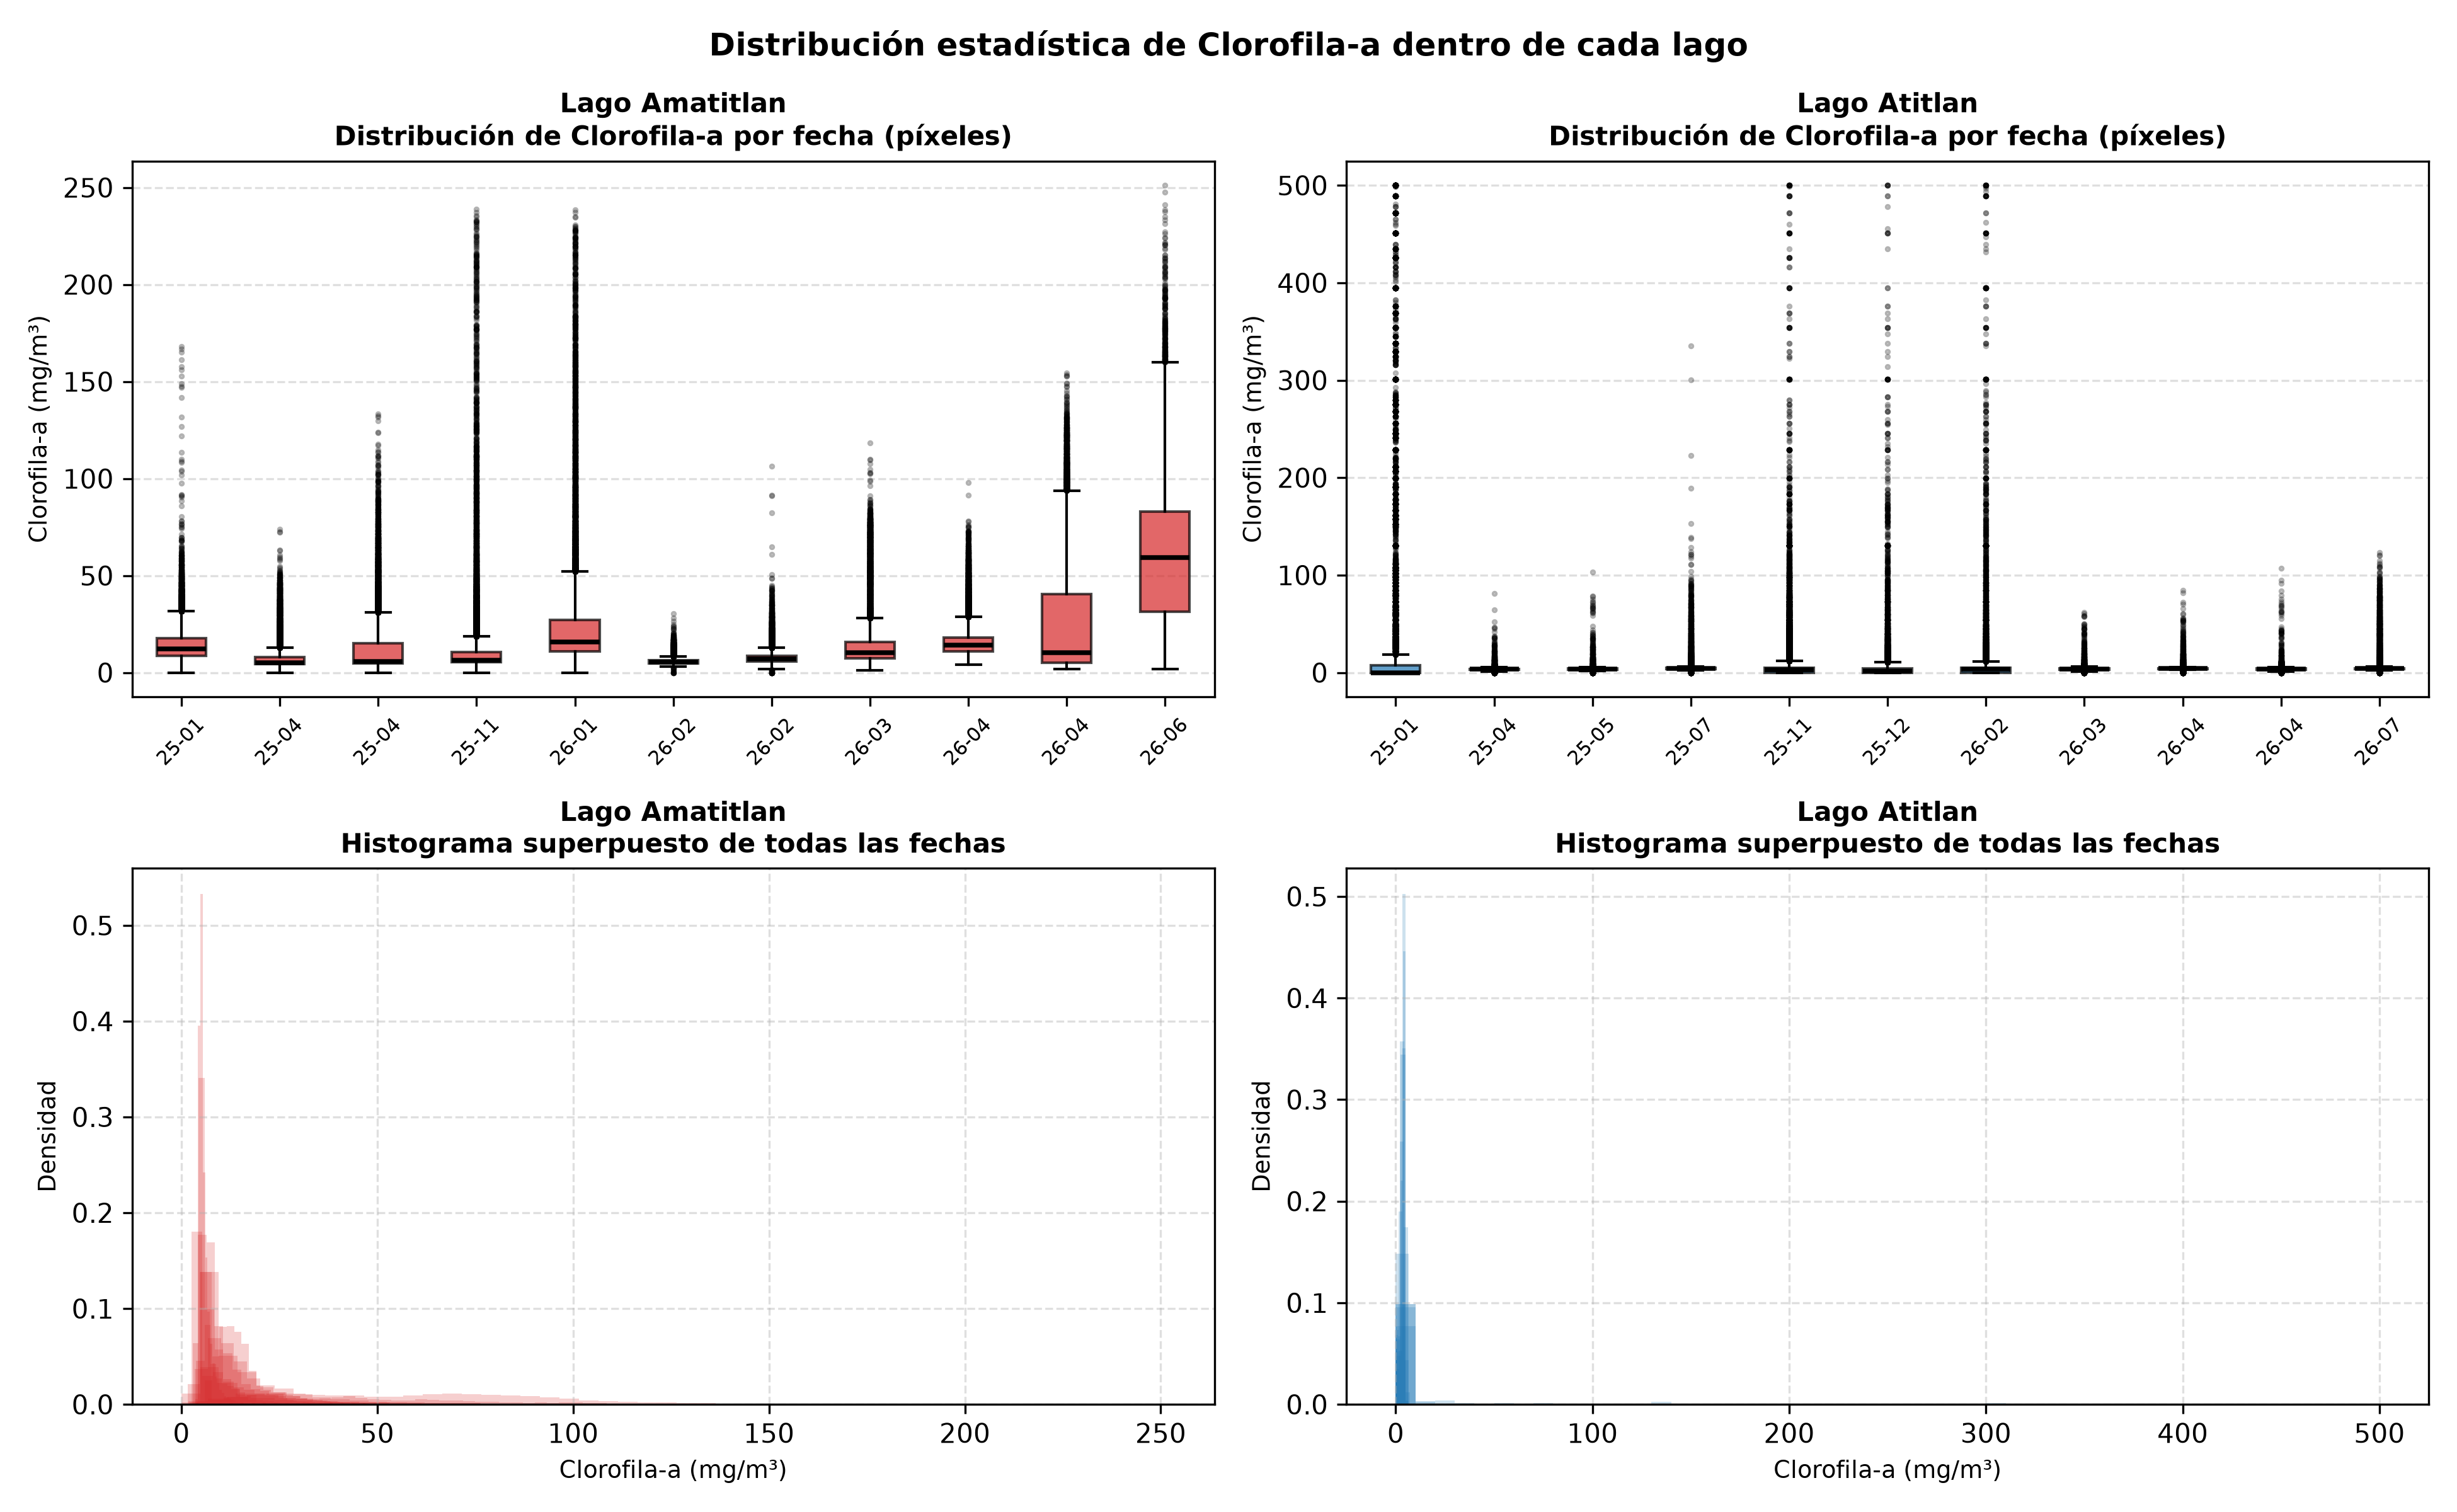
\includegraphics[width=0.92\textwidth]{distribucion_boxplot_hist.png}
    \caption{Distribuci\'on de la clorofila-a por fecha (diagramas de caja, arriba) e histogramas superpuestos de todas las fechas (abajo), para Amatitl\'an (izquierda) y Atitl\'an (derecha).}
    \label{fig:distribucion}
\end{figure}

La distribuci\'on de valores dentro de Amatitl\'an es, en casi todas las fechas, asim\'etrica hacia la derecha: hay muchos p\'ixeles con valores moderados y una cola de p\'ixeles con valores altos que ``estira'' el promedio hacia arriba. En el evento de floraci\'on total (2026-06-19) esa distribuci\'on se vuelve mucho m\'as uniforme, consistente con lo observado antes: ah\'i la floraci\'on ya no es un fen\'omeno de algunos p\'ixeles, sino de todo el lago. En Atitl\'an, la distribuci\'on es siempre angosta y centrada en valores bajos, con colas extremas asociadas a las bah\'ias puntuales, que no logran mover la mediana del lago completo.

\subsection{¿Existe un patr\'on estacional?}

Guatemala tiene una \'epoca seca (noviembre a abril) y una \'epoca lluviosa (mayo a octubre) bien marcadas. Se compar\'o la clorofila-a promedio entre ambas \'epocas para cada lago.

\begin{figure}[H]
    \centering
    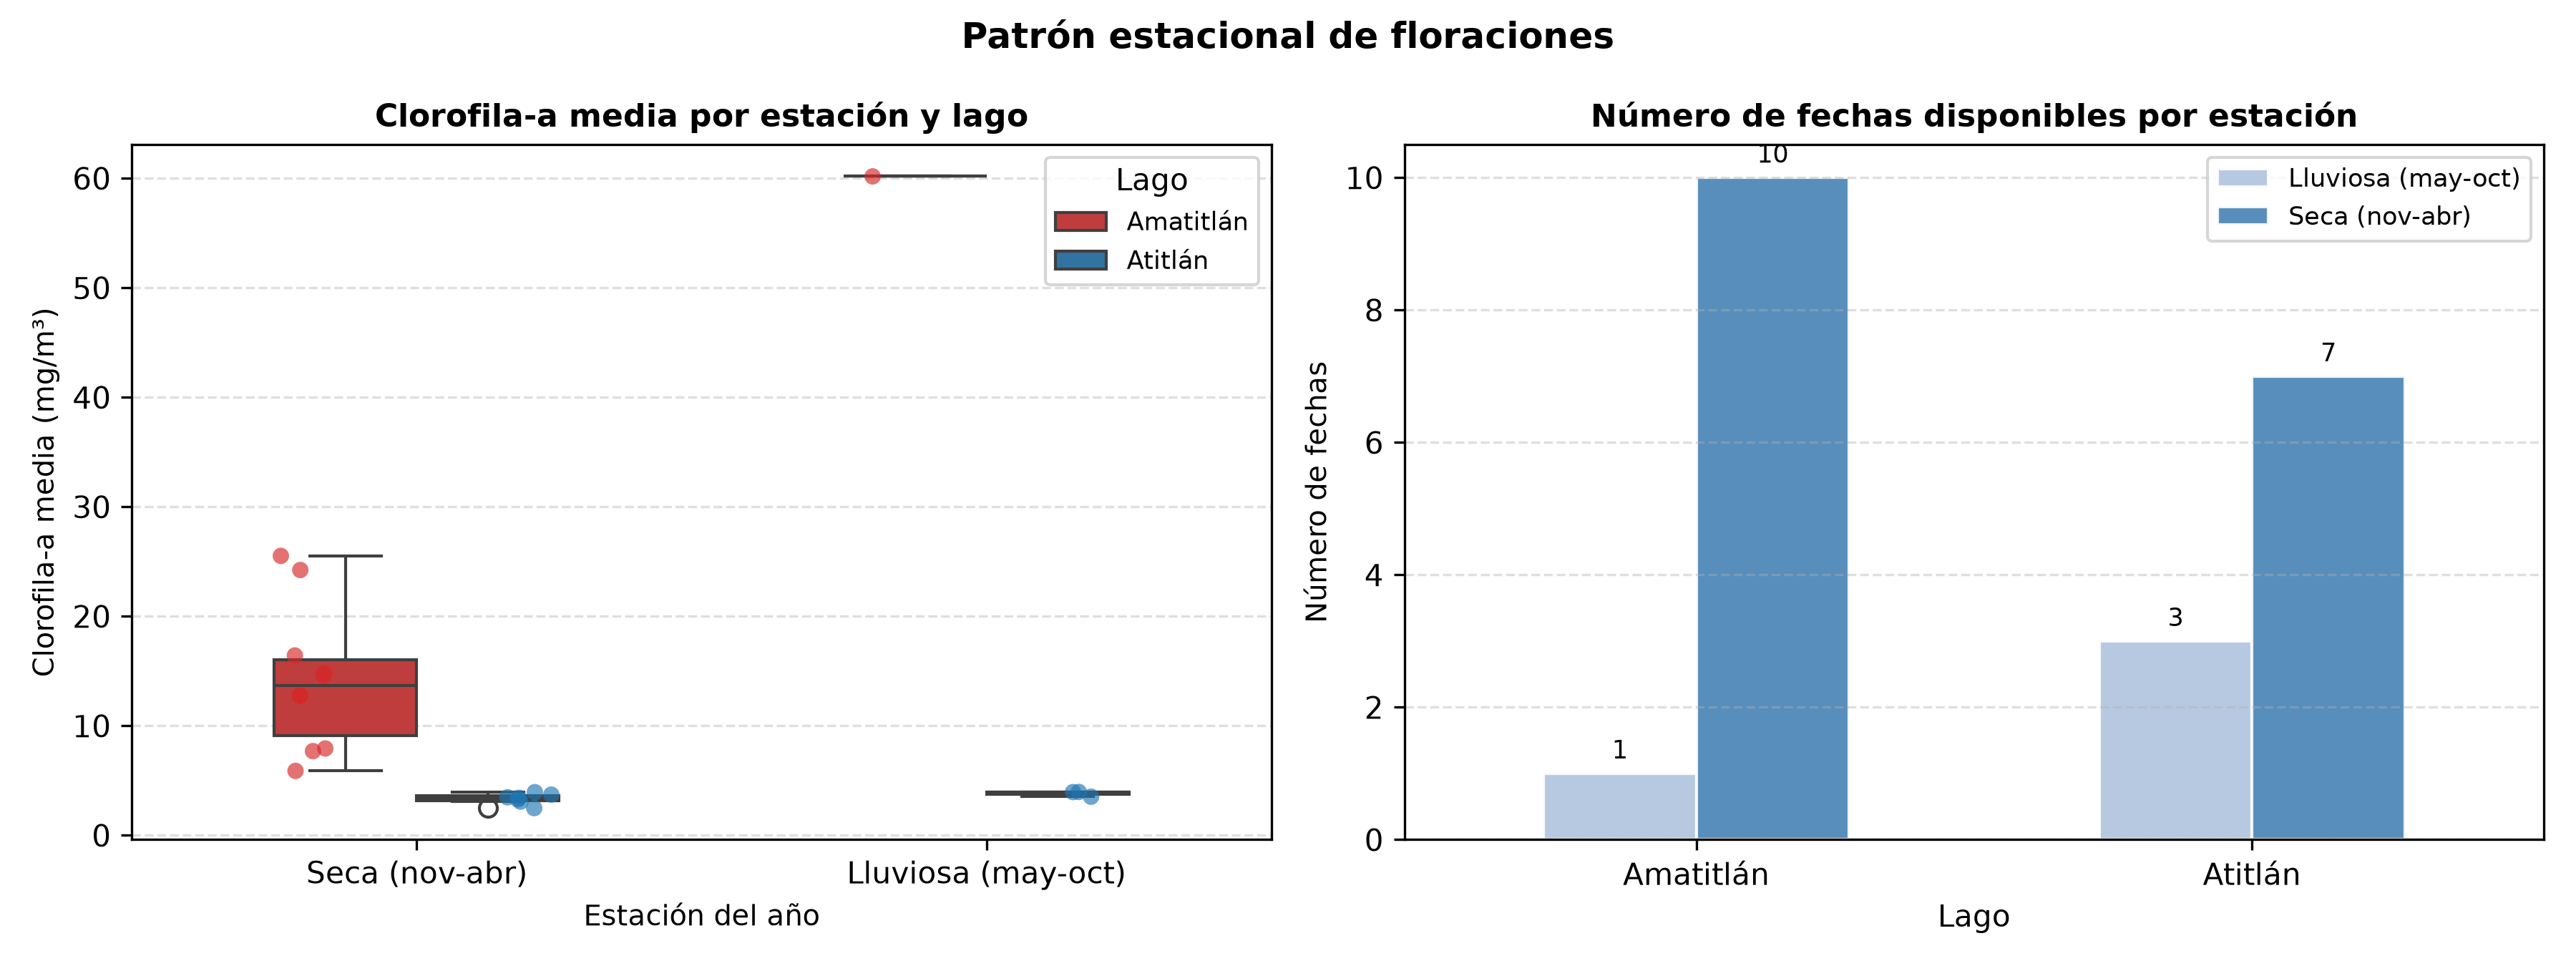
\includegraphics[width=0.92\textwidth]{patron_estacional.png}
    \caption{Clorofila-a media por \'epoca del a\~no y lago (izquierda) y n\'umero de fechas disponibles por \'epoca y lago (derecha).}
    \label{fig:estacional}
\end{figure}

La direcci\'on del efecto es la esperada: en ambos lagos, la clorofila-a promedio es mayor en \'epoca lluviosa que en \'epoca seca. Sin embargo, hay que leer este resultado con cautela: en Amatitl\'an, la \'epoca lluviosa qued\'o representada por una \'unica fecha dentro de las 11 oficiales (justamente 2026-06-19, el pico del per\'iodo), as\'i que esa comparaci\'on estacional en realidad describe un solo evento y no un promedio estacional robusto. En Atitl\'an, la diferencia entre \'epocas es peque\~na (alrededor de 14\,\% m\'as en lluviosa) y queda dentro de la variabilidad normal observada entre fechas. Confirmar un patr\'on estacional real requerir\'ia un muestreo mensual m\'as balanceado a lo largo de varios a\~nos, algo que escapa al alcance de este laboratorio.

% ======================================================================
\section{Conclusiones}
% ======================================================================

\begin{itemize}
    \item El monitoreo satelital con Sentinel-2, combinado con el \emph{Cyano Detection Script} de Sentinel Hub, permiti\'o construir una serie temporal y espacial confiable del estado de ambos lagos sin necesidad de muestreos f\'isicos frecuentes, usando solo las bandas espectrales estrictamente necesarias.
    \item \textbf{Amatitl\'an} se encuentra en un estado de eutrofizaci\'on cr\'onica: su clorofila-a nunca baj\'o de 5.9 mg/m\textsuperscript{3} en el per\'iodo analizado, y en junio de 2026 sufri\'o una floraci\'on que cubri\'o cerca de tres cuartas partes de su superficie. El foco persistente se ubica junto a la desembocadura del r\'io Villalobos, lo que apunta directamente a la carga de nutrientes proveniente del \'area metropolitana de la Ciudad de Guatemala.
    \item \textbf{Atitl\'an} se mantiene saludable a nivel de lago completo, con una variaci\'on de apenas 1.6 veces entre su fecha m\'as limpia y su fecha m\'as cargada. No obstante, presenta focos locales intensos y recurrentes en las bah\'ias de Santiago Atitl\'an, San Pedro La Laguna y Panajachel, zonas de mayor actividad humana y tur\'istica, que conviene seguir monitoreando: el gran volumen del lago diluye estos aportes hoy, pero esa capacidad de amortiguamiento no es infinita si la presi\'on sobre esas bah\'ias sigue creciendo.
    \item La relaci\'on entre la clorofila-a y los \'indices NDVI/NDWI no result\'o estad\'isticamente significativa con las 10-11 fechas disponibles por lago, especialmente en Atitl\'an, donde la variaci\'on natural de clorofila-a es muy peque\~na. Ampliar el n\'umero de fechas, o analizar la relaci\'on a nivel de p\'ixel dentro de las bah\'ias con floraciones locales, ser\'ian los siguientes pasos naturales para profundizar este hallazgo.
    \item En conjunto, la comparaci\'on entre ambos lagos ilustra c\'omo la geograf\'ia (profundidad, volumen) y la presi\'on antr\'opica sobre la cuenca (poblaci\'on, uso del suelo, tipo de afluentes) determinan de forma muy directa la salud de un cuerpo de agua, y c\'omo la observaci\'on satelital permite vigilar ambos factores de manera continua y a bajo costo.
\end{itemize}

% ======================================================================
\section*{Referencias}
\addcontentsline{toc}{section}{Referencias}
% ======================================================================

\begin{itemize}
    \item Copernicus Data Space Ecosystem -- Misi\'on Sentinel-2. \url{https://dataspace.copernicus.eu}
    \item Sentinel Hub -- Repositorio de \emph{custom scripts}, incluido el \emph{Cyano Detection Script} (\texttt{cyanobacteria\_chla\_ndci\_l1c}). \url{https://custom-scripts.sentinel-hub.com}
    \item Kravitz, J. \& Matthews, M. (2020). Algoritmo original de detecci\'on de cianobacterias mediante NDCI, en el que se basa el script utilizado en este laboratorio.
    \item Laboratorio 4. An\'alisis de Datos Geoespaciales. CC3084 -- Data Science, Universidad del Valle de Guatemala, Semestre II 2026.
\end{itemize}

\end{document}
